%!TEX TS-program = xelatex
\documentclass[12pt, a4paper, oneside]{extreport}

%%%%%%%%%% Програмный код %%%%%%%%%%
\usepackage{minted}
% Включает подсветку команд в программах!
% Нужно, чтобы на компе стоял питон, надо поставить пакет Pygments, в котором он сделан, через pip.

% Для Windows: Жмём win+r, вводим cmd, жмём enter. Открывается консоль.
% Прописываем easy_install Pygments
% Заходим в настройки texmaker и там прописываем в PdfLatex:
% pdflatex -shell-escape -synctex=1 -interaction=nonstopmode %.tex

% Для Linux: Открываем консоль. Убеждаемся, что у вас установлен pip командой pip --version
% Если он не установлен, ставим его: sudo apt-get install python-pip
% Ставим пакет sudo pip install Pygments

% Для Mac: Всё то же самое, что на Linux, но через brew.

% После всего этого вы должны почувствовать себя тру-программистами!
% Документация по пакету хорошая. Сам читал, погуглите!



%%%%%%%%%% Математика %%%%%%%%%%
\usepackage{amsmath,amsfonts,amssymb,amsthm,mathtools}
\mathtoolsset{showonlyrefs=true}  % Показывать номера только у тех формул, на которые есть \eqref{} в тексте.
%\usepackage{leqno} % Нумерация формул слева



%%%%%%%%%%%%%%%%%%%%%%%% Шрифты %%%%%%%%%%%%%%%%%%%%%%%%%%%%%%%%%
\usepackage[english, russian]{babel} % выбор языка для документа
\usepackage[utf8]{inputenc} % задание utf8 кодировки исходного tex файла
\usepackage[X2,T2A]{fontenc}        % кодировка

\usepackage{fontspec}         % пакет для подгрузки шрифтов
\setmainfont{Linux Libertine O}   % задаёт основной шрифт документа

\usepackage{unicode-math}     % пакет для установки математического шрифта
\setmathfont[math-style=upright]{Neo Euler} % шрифт для математики


%%%%%%%%%% Работа с картинками %%%%%%%%%
\usepackage{graphicx}                  % Для вставки рисунков
\usepackage{graphics}
\graphicspath{{images/}{pictures/}}    % можно указать папки с картинками
\usepackage{wrapfig}                   % Обтекание рисунков и таблиц текстом


%%%%%%%%%% Работа с таблицами %%%%%%%%%%
\usepackage{tabularx}            % новые типы колонок
\usepackage{tabulary}            % и ещё новые типы колонок
\usepackage{array}               % Дополнительная работа с таблицами
\usepackage{longtable}           % Длинные таблицы
\usepackage{multirow}            % Слияние строк в таблице
\usepackage{float}               % возможность позиционировать объекты в нужном месте
\usepackage{booktabs}            % таблицы как в книгах!
\renewcommand{\arraystretch}{1.3} % больше расстояние между строками

% Заповеди из документации к booktabs:
% 1. Будь проще! Глазам должно быть комфортно
% 2. Не используйте вертикальные линни
% 3. Не используйте двойные линии. Как правило, достаточно трёх горизонтальных линий
% 4. Единицы измерения - в шапку таблицы
% 5. Не сокращайте .1 вместо 0.1
% 6. Повторяющееся значение повторяйте, а не говорите "то же"
% 7. Есть сомнения? Выравнивай по левому краю!

%  вычисляемые колонки по tabularx
\newcolumntype{C}{>{\centering\arraybackslash}X}
\newcolumntype{L}{>{\raggedright\arraybackslash}X}
\newcolumntype{Y}{>{\arraybackslash}X}
\newcolumntype{Z}{>{\centering\arraybackslash}X}

% межстрочный отступ в таблице
\renewcommand{\arraystretch}{1.2}


%%%%%%%%%% Графика и рисование %%%%%%%%%%
\usepackage{tikz, pgfplots}  % язык для рисования графики из latex'a


%%%%%%%%%% Гиперссылки %%%%%%%%%%
\usepackage{xcolor}              % разные цвета

% Два способа включить в пакете какие-то опции:
%\usepackage[опции]{пакет}
%\usepackage[unicode,colorlinks=true,hyperindex,breaklinks]{hyperref}

\usepackage{hyperref}
\hypersetup{
	unicode=true,           % позволяет использовать юникодные символы
	colorlinks=true,       	% true - цветные ссылки, false - ссылки в рамках
	urlcolor=blue,          % цвет ссылки на url
	linkcolor=black,          % внутренние ссылки
	citecolor=black,        % на библиографию
	pdfnewwindow=true,      % при щелчке в pdf на ссылку откроется новый pdf
	breaklinks              % если ссылка не умещается в одну строку, разбивать ли ее на две части?
}

%%%%%%%%%% Другие приятные пакеты %%%%%%%%%
\usepackage{multicol}       % несколько колонок
\usepackage{verbatim}       % для многострочных комментариев
\usepackage{cmap}           % для кодировки шрифтов в pdf

% свешиваем пунктуацию
% теперь знаки пунктуации могут вылезать за правую границу текста, при этом текст выглядит ровнее
\usepackage{microtype}

\usepackage{enumitem} % дополнительные плюшки для списков
%  например \begin{enumerate}[resume] позволяет продолжить нумерацию в новом списке

\usepackage{todonotes} % для вставки в документ заметок о том, что осталось сделать
% \todo{Здесь надо коэффициенты исправить}
% \missingfigure{Здесь будет Последний день Помпеи}
% \listoftodos --- печатает все поставленные \todo'шки


%%%% Оформление %%%%%%%
% размер листа бумаги
\usepackage[
paperwidth=160mm,
paperheight=220mm,
headheight=14mm,
left=10mm,
right=10mm,
top=20mm,
bottom=20mm
]{geometry}

\usepackage{indentfirst}       % установка отступа в первом абзаце главы!!!

\usepackage{fancyhdr}

\pagestyle{fancy}
\fancyhf{}
\fancyhead[LE,RO]{\thepage}
\fancyhead[LO]{\leftmark}
\fancyhead[RE]{\rightmark}


\usepackage{setspace}
%\setstretch{1.3}  % Межстрочный интервал
%\setlength{\parindent}{1.5em} % Красная строка.
%\setlength{\parskip}{4mm}   % Расстояние между абзацами
% Разные длины в латехе https://en.wikibooks.org/wiki/LaTeX/Lengths

% \flushbottom                            % Эта команда заставляет LaTeX чуть растягивать строки, чтобы получить идеально прямоугольную страницу
\righthyphenmin=2                       % Разрешение переноса двух и более символов
\widowpenalty=300                     % Небольшое наказание за вдовствующую строку (одна строка абзаца на этой странице, остальное --- на следующей)
\clubpenalty=3000                     % Приличное наказание за сиротствующую строку (омерзительно висящая одинокая строка в начале страницы)
\tolerance=10000     % Ещё какое-то наказание.

\usepackage{bm}
\usepackage{bbm} % шрифт с двойными буквами

% свешиваем пунктуацию
% теперь знаки пунктуации могут вылезать за правую границу текста, при этом текст выглядит ровнее
\usepackage{microtype}

% для эпиграфов
\usepackage{epigraph} 
\setlength\epigraphrule{0pt}
\renewcommand{\textflush}{flushepinormal}

% Внешний вид подписей к картинкам и таблицам
\usepackage[font=small, labelfont=bf]{caption}
\DeclareCaptionLabelSeparator{colon}{\textbf{.} }
\DeclareCaptionLabelFormat{dash}{#1\hspace{.55ex}#2}
\captionsetup[figure]{labelformat=dash}




%%%%%%%%%% Свои команды %%%%%%%%%%
\usepackage{etoolbox}    % логические операторы для своих макросов

% Математические символы первой необходимости:
\DeclareMathOperator{\sgn}{sign}

\DeclareMathOperator*{\argmin}{arg\,min}
\DeclareMathOperator*{\argmax}{arg\,max}

\DeclareMathOperator{\Cov}{Cov}
\DeclareMathOperator{\Var}{Var}
\DeclareMathOperator{\Corr}{Corr}
\DeclareMathOperator{\E}{\mathop{E}}
\DeclareMathOperator{\Med}{Med}
\DeclareMathOperator{\Mod}{Mod}

\DeclareMathOperator*{\plim}{plim}

\newcommand{\const}{\mathrm{const}}        % const прямым начертанием

%% эконометрические сокращения
\def \hb{\hat{\beta}}
\def \hs{\hat{s}}
\def \hy{\hat{y}}
\def \hY{\hat{Y}}
\def \he{\hat{\varepsilon}}
\def \hVar{\widehat{\Var}}
\def \hCorr{\widehat{\Corr}}
\def \hCov{\widehat{\Cov}}

% Греческие буквы
\def \a{\alpha}
\def \b{\beta}
\def \t{\tau}
\def \dt{\delta}
\def \e{\varepsilon}
\def \ga{\gamma}
\def \kp{\varkappa}
\def \la{\lambda}
\def \sg{\sigma}
\def \tt{\theta}
\def \Dt{\Delta}
\def \La{\Lambda}
\def \Sg{\Sigma}
\def \Tt{\Theta}
\def \Om{\Omega}
\def \om{\omega}

% Готика
\def \mA{\mathcal{A}}
\def \mB{\mathcal{B}}
\def \mC{\mathcal{C}}
\def \mE{\mathcal{E}}
\def \mF{\mathcal{F}}
\def \mH{\mathcal{H}}
\def \mL{\mathcal{L}}
\def \mN{\mathcal{N}}
\def \mU{\mathcal{U}}
\def \mV{\mathcal{V}}
\def \mW{\mathcal{W}}

% Жирные штуки
\def \mbb{\mathbb}

\def \RR{\mbb R}
\def \NN{\mbb N}
\def \ZZ{\mbb Z}
\def \PP{\mbb{P}}
\def \QQ{\mbb Q}

% Карточные масти
\DeclareSymbolFont{extraup}{U}{zavm}{m}{n}
\DeclareMathSymbol{\varheart}{\mathalpha}{extraup}{86}
\DeclareMathSymbol{\vardiamond}{\mathalpha}{extraup}{87}


% Команды первой необходимости
\newcommand{\iid}{\mathrel{\stackrel{\rm i.\,i.\,d.}\sim}}  % ну вы поняли...
\newcommand{\fr}[2]{\ensuremath{^#1/_#2}}   % особая дробь
\newcommand{\ind}[1]{\mathbbm{1}_{\{#1\}}} % Индикатор события
\newcommand{\dx}[1]{\,\mathrm{d}#1} % для интеграла: маленький отступ и прямая d

\newcommand{\indef}[1]{\textbf{#1}}     % выделение ключевого слова в определениях

% бульпоинты в списках
\definecolor{myblue}{rgb}{0, 0.45, 0.70}
\newcommand*{\MyPoint}{\tikz \draw [baseline, fill=myblue,draw=blue] circle (2.5pt);}
\renewcommand{\labelitemi}{\MyPoint}

% для нормального распределения
\newcommand{\expp}[1]{ \exp \left( #1 \right)} 
% для прорисовки нормального распределения
\newcommand\gauss[2]{1/(#2*sqrt(2*pi))*exp(-((x-#1)^2)/(2*#2^2))} 



%%%%%%%%%% Теоремы %%%%%%%%%%
\theoremstyle{plain}              % Это стиль по умолчанию.  Есть другие стили.
\newtheorem{theorem}{Теорема}[section]
\newtheorem{result}{Следствие}[theorem]
% счётчик подчиняется теоремному, нумерация идёт по главам согласованно между собой


\theoremstyle{definition}         % убирает курсив и что-то еще наверное делает ;)
\newtheorem*{definition}{Определение}  % нумерация не идёт вообще

\newtheorem{chudo}{Чудо номер}   % Для первой главы



%%%%%%%%%% Список литературы %%%%%%%%%%

%\usepackage[backend=biber,style=chem-acs,sorting=nty]{biblatex}
% style --- стиль оформления библиографии
% backend --- Движок для сборки. Просто пишите сюда biber. Trust me.
% sorting --- Порядок сортировки в списке. nty = сначала по имени, потом по названию, потом по году выхода статьи. В этот же список можно включить 'a' - по алфавиту,


%\addbibresource{bayes.bib} % сюда нужно вписать свой биб-файлик


%%%%%%%%%% Задачи и их решения %%%%%%%%%%%

\usepackage{answers}

\newtheorem{problem}{\color{myblue} Упражнение}
\Newassociation{sol}{solution}{solution_file}
% sol --- имя окружения внутри задач
% solution --- имя окружения внутри solution_file
% solution_file --- имя файла в который будет идти запись решений
% можно изменить далее по ходу

\setlength{\epigraphwidth}{0.5\textwidth}

\usepackage{pgf,tikz}
\usepackage{mathrsfs}
\usetikzlibrary{arrows}

\begin{document}

%\Opensolutionfile{solution_file}[solutions1]


\chapter{ Что такое Баесовский подход и кому он сдался }

\epigraph{When the facts change, I change my mind. What do you do, sir?}{John Maynard Keynes}


В предыдущей главе мы попытались на простых примерах вникнуть в байесовскую философию и понять что же в ней такого особенного. Никакой глубокой математики мы при этом не использовали. Пора исправить это небольшое упущение и вникнуть в проблему на новом уровне.

\section{Новый шаг вглубь байесовской норы}

До того, как мы открыли эту книгу, нам часто приходилось оценивать различные параметры. Для этого в нашем арсенале находилось довольно большое количество методов. Мы  использовали в повседневной жизни метод максимального правдоподобия, метод моментов, самые разные методы наименьших квадратов\footnote{Было бы интересно узнать как много МНК знает читатель. Одному из авторов на ум прямо сейчас приходит около 10 разных методов.} и даже различные более сложные методы вроде обобщённого метода моментов (GMM). Все эти методы относятся к частотной статистике.

Используя их, мы предполагали, что:

\begin{enumerate}
\item у нас есть какой-то детерминированный неизвестный параметр $\beta$, который нужно оценить;
\item у  нас есть данные $y_1, \ldots, y_n$, связанные с этим параметром;
\item у нас есть модель, которая описывает как наблюдение $y_i$ зависит от параметра $\beta$;
\item у нас есть методы, которые позволяют получить оценку $\hb(y_1, \ldots, y_n)$;
\item полученная нами оценка является случайной величиной, так как она является функцией от наблюдений, то есть \indef{статистикой};
\item у нас есть ряд теорем (ЦПТ, дельта-метод и другие), которые говорят нам о том как распределена случайная величина $\hb$, как для неё можно оценить дисперсию, $\hVar(\hb)$, и построить доверительный интервал;
\item на основе этих теорем мы можем проверять свои гипотезы, связанные с параметром $\beta$ и получать крутые (или не очень)  результаты. 
\end{enumerate}

Грубо говоря, каждый раз, исследуя различные явления, мы шли по такой, отработанной несколькими поколениями статистиков методологии и получали некоторый результат.

При всём этом нам безумно сильно, в силу человеческой любознательной природы, хотелось бы получить ответ, например, на вопрос: <<Какова вероятность того, что $\beta$ больше трёх, $\PP(\beta > 3 \mid y_1, \ldots, y_n)$?>>, но в силу того что $\beta$ является неизвестной константой, получить ответ на этот довольно естественный вопрос мы не могли.

Для того, чтобы выкрутиться из сложившейся ситуации, мы формулировали гипотезу $ H_0 : \beta = 3 $ против альтернативной гипотезы $ H_1 : \beta > 3.$

За кадром мы формулировали  несколько теорем, порождающих критерий для проверки этой гипотезы и некоторые условия, при которых его можно было бы использовать. Статистика для проверки гипотезы, при её верности имела какое-то распределение. Меткое попадание наблюдаемого значения в критическую область говорило нам о том, что $\beta$ значимо отличается от трёх, но при этом оно ничего не могло  рассказать о существенности этого различия. Понятия статистической значимости и смысловой существенности в этой неестественной, дробящей студенческий мозг при изучении, процедуре смешались в единое целое.

У многих опытных читателей, скорее всего, в голове промелькнула мысль: <<Как так? Я же могу оценить вероятность $\hat{\PP} ( \hb > 3)$!>>.  Да, можете, но это оценка вероятности для оценки. А нам хотелось бы работать с истинным значением $\b$.

Кроме того, в частотном подходе мы ставим перед собой только одну гипотезу и производим её проверку. Все остальные существующие гипотезы мы отбрасываем. Обычно это оправдывается методом максимального правдоподобия, который оценивает параметр, стараясь максимизировать вероятность появления выборки. Мы не отвергаем гипотезу $H_0$, если значение правдоподобия при замене параметра $\hb_{MLE}$ на тройку изменяется незначительно.

Байесовцы, в свою очередь, говорят, что никогда точно неизвестно, какая из гипотез верна, и поэтому нельзя просто выбирать одну гипотезу из огромной кучи и тестировать её. Нужно вычислить апостериорную вероятность каждой возможной гипотезы и при прогнозировании учесть всё. Сумма вероятностей всех возможных гипотез равна единице, поэтому, если какая-то гипотеза становится вероятнее, вероятность других уменьшается. Байесовский подход вынуждает таскать за собой множество гипотез вместо одной. И для человека это довольно тяжело. Это было одной из причин того, почему байесовский подход не был раньше популярен. Сегодня благодаря мощным компьютерам таскать за собой целые распределения стало менее проблематично и интерес к байесовскому подходу начал расти.

Внимательный читатель, падкий на красивые идеи, уже усвоил, что философия байесовского подхода позволяет взглянуть на мир под другим углом. Давайте не будем разделять между собой $\hb$ и $\beta$, а всё наше незнание о параметре $\beta$ мы будем формулировать в виде \indef{априорного закона} распределения. Параметр $\beta$ будет случайной величиной, а не константой.

После того, как мы сформировали наше мнение, соберём кучу наблюдений и с помощью формулы Байеса пересчитаем априорное распределение параметра $\beta$ в \indef{апостериорное}

\[ f(\beta \mid y) = \frac{ f(y \mid \beta) \cdot f(\beta)}{f(y)}.\]

На выходе мы получаем целое распределение $f(\beta \mid y)$. Это гораздо больше, чем точечная оценка параметра. Используя его можно получить ответы на любые, интересующие нас вопросы, в том числе измерить вероятность того, что $\beta$ принимает значение больше трёх. Эта вероятность и будет отражать существенность эффекта.

Важно отметить, что байесовский подход --- это другой подход к оцениванию параметров, а не другая модель. В его рамках можно изучать любые классические модели. Изменения касаются способа моделирования неизвестных параметров.

Изобразим всё вышесказанное в виде красивой таблички под номером \ref{bayes_table} и расположим её на странице \pageref{bayes_table}. Надеемся, что это удовлетворит страсть нашего читателя к структурированию новой информации.

\begin{table}
\begin{tabularx}{\textwidth}{L|L}
\hline
{\large Частотный подход} \newline раньше его называли классическим  & {\large Байесовский подход} \newline скоро его будут называть классическим  \\
\hline
\begin{itemize}
\item $\beta$ --- неизвестный параметр, константа
\item Данные: $y_1, \ldots, y_n$
\item Модель: описывает связь $y_i$~с~$\beta$
\item Методы: ML, OLS, GM и т.п. \[\Rightarrow \hb(y_1,\ldots,y_n)\]
\item Теоремы: ЦПТ, дельта-метод и т.п.  \[\Rightarrow \hVar(\hb), \quad \b \in [\hb_L; \hb_H]\]
\item Прогнозы и гипотезы
\end{itemize}

&  % Новый столбец!

\begin{itemize}
\item Нет разделения между $\beta$ и $\hb$
\item Априорное распределение: $ f( \b )$ выражает моё незнание о~$\b$
\item Данные: $y_1, \ldots, y_n$
\item Модель: описывает связь $y_i$~с~$\beta$
\item Апостериорное~распределение:  $f( \b \mid y_1 \ldots y_n )$ получаем байесовским пересчётом
\item В качестве точечной оценки для $\b$ можно взять апостериорную медиану, апостериорное математическое ожидание, апостериорную моду или любой другой апостериорный квантиль
\item Можно построить байесовский интервал (credible or baessian interval), $\PP( \b \in [\b_L ; \b_H]) = 0.95 $
\item Можно получить распределение $\hat y_{n+1}$
\end{itemize}

\\
\end{tabularx}
\caption{Красивая таблица, которая призвана удовлетворить страсть нашего вдумчивого читателя к структурированию новой информации.} \label{bayes_table}
\end{table}

\textbf{Ещё раз, ещё раз!} Мы не знаем параметр $\beta$. Степень своего незнания мы представляем в виде априорного закона распределения. После мы собираем выборку и с помощью обычной формулы условной вероятности делаем пересчёт. Вот и вся любовь. Попробуем заняться этой, новой для нас любовью, на каком-нибудь простом примере.

\section{О карасях, рыбалке и бабушках}

Рассмотрим простой пример. Пусть в озере живут караси и щуки. Петя, живущий в деревне по соседству, выловил в нём карася, щуку и ещё одного карася, а после серьёзно задумался о том с какой вероятностью, $p$, он таскает карасей из озера. Петя предполагает, что в озере настолько много рыбы, что вылов одного карася несильно меняет вероятность поймать нового карася, т.е. наблюдения $y_1 = 1, y_2 = 0, y_3 = 1$ независимы и одинаково распределены.

\subsection*{О том какие у бабушек бывают распределения}

Если бы Петя был частотным статистиком, то он бы воспользовался методом максимального правдоподобия или методом наименьших квадратов и нашёл бы оценку требуемой вероятности. Тем не менее, в родной деревне Пети широко практикуется байесовское воспитание, в связи с чем ему не хотелось бы пользоваться стандартными методами.

Идея! Мы ничего не знаем о параметре $p$. Давайте опишем наше незнание с помощью какой-то априорной функции распределения. Важно  помнить, что на данные при этом смотреть нельзя. Наши априорные ожидания никак не должны быть с ними связаны. В случае Пети, он сначала должен задать распределение $p$, а уже после идти таскать рыб. 

Например, если мы вообще ничего не знаем о том, что происходит в пруду, то логично взять в качестве априорного распределения равномерное, $p \sim \mU[0;1]$. Тем самым мы не только скажем, что настолько ничего не знаем о параметре $p$, что допускаем абсолютно любое значение этого параметра, но и одновременно с этим откинем все невозможные значения, ограничив $p$ отрезком от $0$ до $1$.

\begin{figure}[H]
\begin{minipage}[H]{0.39\linewidth}
\begin{center}
\[ f(p) = \begin{cases}
             1&, p \in [0;1] \\
             0&, \text{иначе}\\
            \end{cases} \]
\end{center}
\end{minipage}
\hfill
\begin{minipage}[H]{0.59\linewidth}
\begin{center}
\begin{tikzpicture}
% оси
\draw [->] (-3.8,0) -- (4,0);
\draw [->] (0,0) -- (0,3.5);
% график
\draw [blue, thick, domain=0:2] plot (\x, 2);
\draw [->, blue, thick] (-3.8,0)--(-0.05,0);
\draw [<-, blue, thick] (2.05,0)--(4,0);
\draw [blue, thick,dashed] (2,0)--(2,2);
% точки
\draw[fill,blue] (2,2) circle [radius=0.03];
\draw[fill,blue] (0,2) circle [radius=0.03];
% подписи
\node [below] at (0,0) {0};
\node [below] at (2,0) {1};
\node [left] at (0,2) {1};
\node [below right] at (4,0) {$p$};
\node [left] at (0,3.3) {$f(p)$};
\end{tikzpicture}
\end{center}
\end{minipage}
\end{figure}

В то же самое время, если у нас есть любящая порыбачить (а заодно и внука) бабушка, которая говорит, что за свою жизнь выловила из озера карасей в два раза больше, чем щук, то вполне логично поверить ей и предположить, что у параметра $p$ будет распределение с плотностью

\begin{figure}[H]
\begin{minipage}[H]{0.39\linewidth}
\begin{center}
\[ f(p) = \begin{cases}
            2p&, p \in [0;1] \\
             0&, \text{иначе.}\\
            \end{cases} \]
\end{center}
\end{minipage}
\hfill
\begin{minipage}[H]{0.59\linewidth}
\begin{center}
\begin{tikzpicture}[scale=0.8]
% оси
\draw [->] (-3.8,0) -- (4,0);
\draw [->] (0,0) -- (0,4.5);
% график
\draw [blue, thick, domain=0:2] plot (\x,2*\x);
\draw [->, blue, thick] (-3.8,0)--(-0.05,0);
\draw [<-, blue, thick] (2.05,0)--(4,0);
\draw [blue, thick,dashed] (2,0)--(2,4);
\draw [blue, thick,dashed] (0,4)--(2,4);
% точки
\draw[fill,blue] (2,4) circle [radius=0.03];
\draw[fill,blue] (0,4) circle [radius=0.03];
% подписи
\node [below] at (0,0) {0};
\node [below] at (2,0) {1};
\node [left] at (0,4) {2};
\node [below right] at (4,0) {$p$};
\node [above left] at (0,4.3) {$f(p)$};
\end{tikzpicture}
\end{center}
\end{minipage}
\end{figure}


Тогда в своих априорных предположениях мы учтём многолетний опыт бабушки, а вместе с ним большое число случайных выборок из местного прудика, которые мы не видели. Если бабушка не врёт, и в пруду ничего с тех пор не поменялось, дополнительная информация поможет нам получить более точные оценки. Однако, если бабушка Пети никогда не ловила рыбу (или это вообще не его бабушка, хотя она и утверждает обратное), то принимать её априорное мнение о рыбе на веру ни в коем случае нельзя. Как уже отмечалось выше, вы должны быть готовы сделать на своё априорное мнение денежную ставку. 

Давайте посмотрим что у нас получится при разных априорных мнениях. Пусть $p \sim \mU[0;1]$. Найдём апостериорную плотность распределения параметра $p$. Воспользуемся формулой Байеса:

\[ f(p \mid y_1,y_2,y_3) = \frac{f(p,y_1,y_2,y_3)}{f(y_1,y_2,y_3)} = \frac{f(y_1,y_2,y_3 \mid p) \cdot f(p)}{f(y_1,y_2,y_3)}.\]

В знаменателе полученной дроби стоит значение совместной плотности распределения трёх случайных величин в точке $y_1, y_2, y_3$. Это какая-то константа. Пренебрежём ей для лёгкости расчётов. Чуть позже мы восстановим её назад. С помощью значка $\propto$ будем записывать равенство с точностью до константы

\[  \frac{f(y_1,y_2,y_3 \mid p) \cdot f(p)}{f(y_1,y_2,y_3)} \propto f(y_1,y_2,y_3 \mid p) \cdot f(p).\]

Вспоминаем о том, что собранные нами наблюдения независимы (что довольно наивно)\footnote{Упорный читатель поймёт эту шутку в следующей главе} и получаем

\begin{multline*}
f(y_1,y_2,y_3 \mid p) \cdot f(p) =  f(y_1 \mid p) \cdot f(y_2 \mid p) \cdot f(y_3 \mid p) \cdot f(p) = \\ = \PP(y_1 = 1 \mid p) \cdot \PP(y_2 = 0 \mid p) \cdot \PP(y_3 = 1 \mid p) \cdot f(p) = p \cdot (1 - p) \cdot p \cdot 1.
\end{multline*}

Выходит, что апостериорная плотность распределения параметра $p$ должна иметь вид

\[ f(p \mid y_1, y_2, y_3) = const \cdot p^2 \cdot (1-p).\]

Осталось восстановить нормировочную константу. Вспоминаем, что интеграл по области определения апостериорной плотности распределения должен быть равен единице


\[ const \cdot \int_0^1 p^2 \cdot (1-p) \dx{p}  = 1 \quad \Rightarrow \quad const = 12 \]

Итак, ваши авации! Апостериорное распределение параметра $p$:


\[ f(p \mid y_1, y_2, y_3) =
  \begin{cases}
    12 \cdot p^2 \cdot (1-p)   & \quad p \in [0;1] \\
    0      & \quad \text{иначе}\\
  \end{cases}
\]


\begin{figure}[H]
\begin{minipage}[H]{0.49\linewidth}
\center Априорное распределение: \\[2.5ex]
\begin{tikzpicture}
% оси
\draw [->] (-1.8,0) -- (4,0);
\draw [->] (0,0) -- (0,3.5);
% график
\draw [blue, thick, domain=0:2] plot (\x, 2);
\draw [->, blue, thick] (-1.8,0)--(-0.05,0);
\draw [<-, blue, thick] (2.05,0)--(4,0);
\draw [blue, thick,dashed] (2,0)--(2,2);
% точки
\draw[fill,blue] (2,2) circle [radius=0.03];f
\draw[fill,blue] (0,2) circle [radius=0.03];
% подписи
\node [below] at (0,0) {0};
\node [below] at (2,0) {1};
\node [left] at (0,2) {1};
\node [below right] at (4,0) {$p$};
\node [left] at (0,3.3) {$f(p)$};
\end{tikzpicture}
\end{minipage}
\hfill
\begin{minipage}[H]{0.49\linewidth}
\center Апостериорное распределение: \\[2.5ex]
\begin{tikzpicture}
% оси
\draw [->] (-1.8,0) -- (3,0);
\draw [->] (0,0) -- (0,3.5);
% график12
\draw [blue, thick, domain=0:1] plot (\x, {12*\x*\x*(1-\x)});
\draw [blue, thick] (-1.8,0)--(0,0);
\draw [blue, thick] (1,0)--(3,0);
%\draw [blue, thick,dashed] (2,0)--(2,2);
% точки
%\draw[fill,blue] (2,2) circle [radius=0.03];
%\draw[fill,blue] (0,2) circle [radius=0.03];
% подписи
\node [below] at (0,0) {0};
\node [below] at (1,0) {1};
% \node [left] at (0,1) {1};
\node [below right] at (3,0) {$p$};
\node [left] at (0,3.3) {$f(p)$};
\end{tikzpicture}
\end{minipage}
\end{figure}

В априорном мнении Петя не знал где находится $p$ и все точки для него были одинаково предпочтительны. Апостериорное мнение говорит, что вероятность поймать карася гораздо ближе к единице, чем к нулю. Проделаем те же самые рассуждения, но уже учитывая априорное мнение бабушки.

По аналогии получаем

\[ f(p \mid y_1, y_2, y_3) = const \cdot p^2 \cdot (1-p) \cdot 2p = const \cdot p^3 \cdot (1-p).\]

Восстанавливаем константу:

\[ const \cdot \int_0^1 p^3 \cdot (1-p) \dx{p}  = 1 \quad \Rightarrow \quad const = 20.\]

Снова получаем апостерирную функцию плотности

\[ f(p \mid y_1, y_2, y_3) =
  \begin{cases}
    20 \cdot p^3 \cdot (1-p)   & \quad p \in [0;1] \\
    0      & \quad \text{иначе.}\\
  \end{cases}
\]

\begin{figure}[H]
\begin{minipage}[H]{0.49\linewidth}
\center Априорное распределение: \\[2.5ex]
\begin{tikzpicture}[scale=0.8]
% оси
\draw [->] (-1.8,0) -- (4,0);
\draw [->] (0,0) -- (0,4.5);
% график
\draw [blue, thick, domain=0:2] plot (\x,2*\x);
\draw [->, blue, thick] (-1.8,0)--(-0.05,0);
\draw [<-, blue, thick] (2.05,0)--(4,0);
\draw [blue, thick,dashed] (2,0)--(2,4);
\draw [blue, thick,dashed] (0,4)--(2,4);
% точки
\draw[fill,blue] (2,4) circle [radius=0.03];
\draw[fill,blue] (0,4) circle [radius=0.03];
% подписи
\node [below] at (0,0) {0};
\node [below] at (2,0) {1};
\node [left] at (0,4) {2};
\node [below right] at (4,0) {$p$};
\node [above left] at (0,4.3) {$f(p)$};
\end{tikzpicture}
\end{minipage}
\hfill
\begin{minipage}[H]{0.49\linewidth}
\center Апостериорное распределение: \\[2.5ex]
\begin{tikzpicture}
% оси
\draw [->] (-1.8,0) -- (3,0);
\draw [->] (0,0) -- (0,3.5);
% график12
\draw [blue, thick, domain=0:1] plot (\x, {20*\x*\x*\x*(1-\x)});
\draw [blue, thick] (-1.8,0)--(0,0);
\draw [blue, thick] (1,0)--(3,0);
%\draw [blue, thick,dashed] (2,0)--(2,2);
% точки
%\draw[fill,blue] (2,2) circle [radius=0.03];
%\draw[fill,blue] (0,2) circle [radius=0.03];
% подписи
\node [below] at (0,0) {0};
\node [below] at (1,0) {1};
% \node [left] at (0,1) {1};
\node [below right] at (3,0) {$p$};
\node [left] at (0,3.3) {$f(p)$};
\end{tikzpicture}
\end{minipage}
\end{figure}

Если учесть и мнение бабушки и нашу выборку, то получится, что шансы того, что карасей в озере мало, минимальны.  

Сравним между собой априорную вероятность $\PP( p > 0.5)$ и апостериорную вероятность того, что $\PP( p > 0.5 \mid y_1, \ldots, y_3)$, а также априорное и апостериорное математические ожидания, $\E(p)$ и $\E(p \mid y_1, \ldots, y_3)$.


\begin{table}[H]
\begin{tabularx}{\textwidth}{@{}XX@{}}
\toprule	
Равномерное распределение: & Распределение бабушки: \\
\midrule
$ \PP( p > 0.5 ) = \int_{0.5}^1 1 \dx{p} = 0.5 $  &   $ \PP( p > 0.5 ) = \int_{0.5}^1 2p \dx{p} = 0.75 $ \\
$\PP( p > 0.5 \mid y) \approx 0.68  $& $\PP( p > 0.5 \mid y) =  0.81 $  \\
$\E(p) = \int_0^1 p \cdot 1 \dx{p} = 0.5 $ & $ \E(p) = \int_0^1 p \cdot 2p \dx{p}  \approx 0.66 $  \\
$\E(p \mid y) = \int_0^1 12 \cdot p^3 \cdot (1-p) \dx{p} = 0.6$ & $\E(p \mid y) = \int_0^1 20  \cdot p^4 \cdot (1-p) \dx{p} \approx 0.66$ \\
\bottomrule
\end{tabularx}
\end{table}


Видим, что в первой ситуации вероятность того, что карасей больше чем щук, при учёте наблюдений увеличивается. Ровно как и доля карасей. Во втором случае, грубо говоря,  мои наблюдения подтверждают мнение бабушки и математическое ожидание не изменяется. По той же причине вероятность того, что карасей больше чем щук увеличивается ещё сильнее. 

Кстати говоря, иногда возникают ситуации, в которых апостериорный результат не зависит от того, во что мы верим. Это говорит о том, что у нас очень много данных и взаимосвязь в них прослеживается достаточно чётко. 

\textbf{Ещё раз, ещё раз!} 

\begin{itemize}
\item  априорное распределение выбирается до сбора данных;
\item  с помощью априорного распределения мы пытаемся описать своё незнание;
\item  оно отбрасывает заведомо неверные значения параметра;
\item  вы должны быть готовы сделать денежную ставку на выбранное вами априорное распределение;
\item  на выходе мы получаем целое апостериорное распределение, с помощью которого можем отвечать на разные вопросы.
\end{itemize}

\subsection*{О точечных оценках} 

Мы получаем на выходе гораздо больше, чем просто точечную оценку. В конечном итоге вся информация о параметре $p$ содержится в его апостериорном распределении, с помощью которого можно отвечать на любые вопросы, касающиеся этого параметра. 

Тем не менее, если от нас требуют точечную оценку, в качестве неё мы могли бы использовать, математическое ожидание, моду или медиану. Конкретный выбор зависит от того как именно нас накажу за то, если мы ошибёмся. Выбор $\beta_F$ зависит от выбранной функции потерь. Вспомните, что происходило с красавицей в одном из чудес первой главы. Она выбирала в зависимости от системы наград и наказаний. 

Так, например, если мы угадали параметр, то в награду получаем половину царства и принцессу, а если не угадали, то нам отрубают голову, выгоднее всего для нас назвать самое вероятное значение параметра, то есть моду апостериорного распределения. 

Если функция потерь квадратичная, $(\beta_F - \beta)^2$, у нас отнимают площадь царства (и, возможно, площадь принцессы) пропорциональную квадрату отклонения спрогнозированного нами значения от настоящего, то выгоднее всего назвать в качестве оценки математическое ожидание апостериорного распределения.

Если функция потерь абсолютная, $|\beta_F - \beta|$, то в качестве оценки выгодна медиана. Выбор функции потерь, в свою очередь, зависит от поставленной перед нами задачи.

На самом деле, байесовский подход позволяет анализировать различные функции потерь, которые мы можем использовать для обучения моделей, и понимать, что именно мы получаем в качестве прогноза на выходе. Иногда можно даже обнаружить, что функция потерь была нами выбрана не очень удачно. О таких вещах мы обязательно поговорим немного позже, а сейчас для полноты картины найдём для равномерного априорного распределения моду и медиану.

Сконцентрируемся. Закроем глаза и попытаемся отыскать в чертогах разума определения медианы и моды.  Медиана --- это квантиль уровня $0.5$. Иными словами это такое значение случайной величины, что 

\[\PP(p < \Med) = \PP(p > \Med) = 0.5.\]

 Найдём её!

\[ \PP(p > \Med) = 0.5 \quad \Rightarrow \quad \int_0^{\Med} 12 \cdot p^2 \cdot (1-p) \dx{p} = 0.5  \]

Взятие этого интеграла приведёт нас к уравнению четвёртой степени. Нам подойдёт решение $\Med(p) \approx 0.61 $. Скорее всего, слова <<уравнение четвёртой степени>> оставили у впечатлительного  читателя не очень хороший осадок. Про такие сложности и про то как умело на практике их избегают компьютеры мы поговорим в следующей главе. 

Модой непрерывной случайной величины называется такое её значение, при котором плотность распределения достигает локального максимума. Вполне логично, что $\Mod(p) = \frac{2}{3}$:

\[ (12 \cdot p^2 \cdot (1-p) )' = p \cdot (2 - 3 \cdot p) = 0 \quad \Rightarrow \quad p = \frac{2}{3} \vee p = 0.\]

Таким образом мы получили целых три точечные оценки: $0.6, 0.61$ и $0.66$. Как это не странно, они расположены довольно близко друг к другу. По мере увеличения количества наблюдений, пик апостериорного распределения будет становится всё острее, а точечные оценки будут становиться всё ближе.

\subsection*{О доверительных и байесовских интервалах}

Едем дальше. В частотном подходе мы часто делали интервальные оценки, строили доверительные (confidence) интервалы. В байесовском подходе также можно делать интервальные оценки, а именно строить байесовские (bayesian или credible) интервалы. Между доверительным и байесовским интервалом есть тонкая разница. Доверительные интервалы обладают странным свойством. Если мы построили 95\% доверительный интервал, то говорить, что истинное значение параметра $p$ попадает в этот интервал с вероятностью $0.95$ неправильно. Этот интервал накрывает истинное значение параметра с вероятностью 95\%, и он может как содержать его, так и не содержать, но метод построения обеспечивает вероятность накрытия в 95\%. Это связано с тем, что мы работаем при построении интервала не с истинным значением параметра $p$, а с его оценкой $\hat p$. Для байесовского интервала, действительно, вероятность попадания параметра $p$ в него равна $0.95$.

Обычно, нам хотелось получить самые короткие интервалы. Почему самые короткие? Если Петя говорит, что с вероятностью $0.95$ температура завтра будет лежать в интервале от 2 до 5 градусов, а Вася говорит, что от 3 до 10 градусов, ошибаться они будут одинаково, в 5\% случаев, однако точность прогноза будет выше у Пети. Самый короткий байесовский интервал называется \indef{HPD (highest probability density interval)}. Конечно же, можно строить интервалы для любых вероятностей, а не только для $0.95$. 

Отдельно стоит сказать, что при определённых условиях значение функции плотности будет одинаковой на правом и левом конце интервала. Чтобы выяснить когда происходит такая интересная штука, читателю предлагается решить упражнение \ref{upr_conf}.

Для нашего случая, чтобы найти HPD, необходимо решить следующую задачу:

\begin{equation*}
	\left \{
	\begin{aligned}
		&b - a \longrightarrow \min_{a,b} \\
		&\int_a^b 12\cdot p^2 \cdot (1-p) \dx{p} = 0.95. \\
	\end{aligned}
	\right.
\end{equation*}

Можно взять интеграл, получить ограничение $4b^3 - 3b^4 -4a^3 + 3a^4 = 0.95$, не забыть, что $0 \le a,b \le 1$, выписать лагранджиан и получить, что $a \approx 0.23 $, $b \approx0.96 $. При этом, значение плотности апостериорного распределения в точке $a$ совпадёт для нашего случая с её значением в точке $b$. Зная факт из упражнения \ref{upr_conf}, можно было бы воспользоваться тем, что $f(a) = f(b)$ и найти доверительный интервал из задачи

\begin{equation*}
	\left \{
	\begin{aligned}
		&b - a \longrightarrow \min_{a,b} \\
		&f(a) = f(b).  \\
	\end{aligned}
	\right.
\end{equation*}

Те читатели, которые не выпали из повествования после слов <<уравнение четвёртой степени>>, легко могли выпасть сейчас. Однако спешу обрадовать, на практике все вычислительные сложности на себя берёт компьютер, и здесь все эти примеры находятся лишь для того, чтобы показать где именно возникают проблемы.

\subsection*{О прогнозах} 

Когда мы строим какую-то модель, мы хотим на выходе получить прогноз. В данном случае нам было бы безумно интересно получить ответ на вопрос, какая рыба будет выловлена в озере следующей. Логично, что если у нас есть апостериорное распределение параметра $p$, то прогнозом будет какое-то распределение для нового значения $y$. Наш прогноз не будет точечным. Дело осталось за малым, преобразовать $f(b \mid y)$ в $\PP(y_4 = \text{карась} \mid y)$. Сделаем это несколькими способами.

\textbf{Способ первый, безынтегральный:} мы знаем, что повторное математическое ожидание убирает условие, то есть 

\[ \E(Z) = \E( \E(Z \mid W)). \] 

 Если случайная величина $Z$ принимает значения $0$ и $1$, тогда

\[  \PP(Z = 1) = \E(Z) = \E( \PP( Z = 1 \mid W)). \]

Более того, если есть какое-то дополнительное условие $A$, тогда выполнится 

 \[ \PP(Z=1 \mid A) = \E(\PP(Z = 1 \mid W,A) \mid A).\]

Чтобы осознать это, будем индексом под математическим ожиданием указывать относительно какого распределения мы ищем это математическое ожидание. В первой ситуации мы искали математическое ожидание относительно $\PP$, значит

 \[ \E_{\PP}(Z) = \E_{\PP}(\E_{\PP}(Z|W)).\]

Если мы рассмотрим $\PP(Z=1 \mid A)$, то мы, сказав что наступило событие $A$, наложим на изначальное пространство элементарных исходов какое-то ограничение и перейдём к новой вероятностной мере $\PP_A$, для которой также выполняется

\[ \E_{\PP_A}(Z) = \E_{\PP_A}(\E_{\PP_A}(Z \mid W)) \].

Но что такое $\PP_A$? Это ничто иное, как условная вероятность некоторого события, $\PP(\mbox{ } \ldots \mid A)$. Делаем везде замену и получаем, что

\[\E_{\PP}(Z \mid A) = \E_{\PP}(\E_{\PP}(Z \mid W, A)\mid A).\]

Вернёмся к задаче и применим к ней этот интересный факт:

\begin{multline*}
 \PP(y_4 = \text{карась} \mid y_1,y_2,y_3) = \\ =  \E( \PP( y_4 = \text{карась} | p,y_1,y_2,y_3) \mid y_1,y_2,y_3) = \\ =  \E(p \mid y_1,y_2,y_3) = 0.6.
\end{multline*}

Такой хитрый способ найти прогноз не является универсальным. Поэтому посмотрим на интегралы, которые помогают сделать это в общем случае. 

\textbf{Способ второй, хитро-интегральный:} распишем искомую вероятность по формуле условной вероятности. 

\begin{multline*}
\PP(y_4 = \text{карась} \mid y_1,y_2,y_3) = \\ =  \frac{\PP(y_1 = \text{карась},y_2 = \text{щука},y_3 = \text{карась},y_4 = \text{карась})}{\PP(y_1 = \text{карась},y_2 = \text{щука},y_3 = \text{карась})} = ^*
\end{multline*}

Найти ни верхнюю вероятность ни нижнюю в силу того, что $y_1, y_2, y_3,y_4$ и $p$ являются случайными величинами, мы не можем. Более того, эти случайные величины зависимы. Случайная величина $p$ влияет на реализацию каждой из этих трёх случайных величин. Выше, мы вскользь вспомнили о чуде, связанном со Спящей Красавицей и её потерями. Сейчас пришло время вспомнить про чудо условной независимости. 

Заметим, что $y_1|p$,  $y_2|p$, $y_3|p$, $y_4|p$ независимые случайные величины, а $\PP(y_1 = \text{карась}) = \E(y_1 = \text{карась} \mid p)$. Воспользуемся этим:

\begin{multline*}
 ^* =  \frac{ \E(\PP(y_1 = 1,y_2 = 0,y_3 = 1,y_4=1 \mid p))}{\E(\PP(y_1 = 1,y_2 = 0,y_3=1 \mid p))} =  \frac{\E(p^3(1-p))}{\E(p^2(1-p))} = \\ =  \frac{\E(p^3) - \E(p^4)}{\E(p^2) - \E(p^3)} =  \frac{\frac{1}{4} - \frac{1}{5}}{\frac{1}{3} - \frac{1}{4}} = \frac{12}{20} = 0.6.
 \end{multline*}

Конечно же для поиска всех математических ожиданий вида $\E(p^k)$ пришлось брать интегралы.

\textbf{Способ третий, интегрально-влобовый:} поговорим о прогнозировании чуть более подробно, в общем, непрерывном случае. В первой главе, когда мы обсуждали чудеса условной вероятности и вспоминали формулы, мы выяснили, что из совместной плотности распределения $f(x,y)$ можно получить частную плотность $f(x)$, выинтригрировав совместную плотность по переменной $y$, а именно 

\[ f(x) = \int f(x,y) \dx{y} = \int f(x \mid y) f(x) \dx{y}.\]  

Мы говорили, что эта формула является аналогом формулы для поиска полной вероятности. Мы перебираем континуальное количество гипотез для переменной $Y$ и находим плотность для $X$.  Раз уж мы начали делать флэшбэки к первой главе, давайте заодно вспомним упражнение 9. Если недобросовестный читатель проигнорировал его, то самое время вернуться назад и разобрать. 

 Будем рассуждать для общего случая. Пусть у нас есть объясняемая переменная $y$ и объясняющая $x$. Что мы сделали? Мы сделали байесовский вывод и получили апостериорную плотность для параметра, 

\[ f(\b \mid x, y) \propto f(y \mid x, \b) \cdot f(\b \mid x).\]

Теперь мы хотим перейти от известной нам апостериорной плотности для параметра $\b$ к плотности для нового значения $y_{new}$, $f(y_{new} \mid x_{new},x,y)$. Выинтегрируем из уже известных нам плотностей лишние части и получим требуемое

\begin{multline*}
f(y_{new} \mid x_{new},x, y) =\int f(y_{new}, \b \mid x_{new}, x,y) \dx{\b} = \\ =  \int f(y_{new} \mid x_{new}, x,y,\b) f(\b \mid x,y) \dx{\b}.
\end{multline*}

\todo[inline]{Это же так? Я боюсь ошибиться в этой части с условиями.} 

Получаем интеграл произведения двух известных нам плотностей. Для случая карасей и щук получаем

\[    
f(y \mid p) = \int f(y \mid p) f(p \mid y) \dx{p} = \int p \cdot f(p \mid y) \dx{p} = \E(p \mid y) = 0.6
\]

Таким образом, получаем требуемое распределение. Вероятность того, что выловлен карась, равна $0.6$. Делая всё это, мы снова сталкиваемся с вычислительными сложностями. Нужно брать интегралы. Повсюду куча интегралов. Решая упражнение с распределением Бернулли и тремя наблюдениями, мы уже накопили кучу вычислительных проблем. Тому как компьютер борется с этими проблемами мы посвятим несколько глав.

Сейчас мы предлагаем читателю закрепить всё то, о чём мы говорили выше и попробовать решить парочку упражнений. В упражнении \ref{upr1}  читателю предлагается сделать пару ставок на априорные распределения. В упражнении \ref{upr2} предлагается сделать байесовский вывод с одним наблюдением и геометрическим распределением. По механике оно повторяет всё то, о чём говорилось выше, однако в нём нет ни лагранджианов, ни чётвертых степеней. 

\section{Распределение Бернулли в общем случае} 

Вы уже решили самостоятельно предложенные выше упражнения? Если нет, бегом решать! Если да, то вы большой молодец и заслуживаете новых интересностей! В этом разделе речь пойдёт про общий случай для распределения Бернулли. Давайте представим себе следущую ситуацию. 

Испанские конкистадоры высадились в Южной Америке. Вместе с собой они привезли кучу интересных прогрессивных европейских вундервафель. Они предлагают индейцам сыграть в следующую игру. Испанцы загадывают одну из сторон монетки. Эрнан Кортес подкидывает её. Если выпадает сторона, загаданная испанцами, то индейцы покидают свои земли. Если выпадает сторона, загаданная индейцами, европейцы отдают им все свои вундервафли и уходят с миром. Старейшины местного племени собрались на совет, на котором каждый из них хотел бы высказать своё мнение о выпадении орла в виде априорного распределения. 

\begin{itemize}
	\item Первый старейшина вообще не знает что такое вероятность.
	\item Второй старейшина не знает что такое монетка, но знает что такое вероятность. 
	\item Третий старейшина однажды видел монетку, он даже вертел её в своих руках и говорит, что, если она сделана хорошо (а скорее всего это так), то будет выпадать с  вероятностью $\frac{1}{2}$. 
	\item Четвёртый старейшина уверен, что монетка у испанцев односторонняя. На ней есть только та сторона, которую выберут испанцы. Какую именно сторону они выберут, он не знает.
	\item Пятый старейшина склонен полагать, что монетка неправильная и та сторона, которую выберут испанцы,выпадает чаще. Какую именно сторону они выберут, он не знает.
\end{itemize}

Попробуйте самостоятельно придумать априорные распределения, а уже после читайте решение. 

Попробуем сформулировать априорные ожидания старейшин на привычном для нас языке. Поскольку первый старейшина не знает что такое вероятность, он может закодировать своё незнание несобственным распределением $\mU [-\infty; +\infty]$. 

Второй старейшина знает что такое вероятность, он знает, что она лежит на отрезке от нуля до единицы. Он своё незнание может выразить как $\mU [0;1]$.

Пик априорного распределения третьего старейшины должен приходиться на $\frac{1}{2}$. Этого можно было бы достичь, используя треугольное распределение.

\begin{figure}[H]
	\begin{minipage}[H]{0.49\linewidth}
		\begin{center}
			\[ f(\beta) = \begin{cases}
			4p &, p \in [0;\frac{1}{2}] \\
			4(1-p) &, p \in [\frac{1}{2};1] \\
			\mbox{ } 0&, \text{иначе}\\
			\end{cases} \]
		\end{center}
	\end{minipage}
	\hfill
	\begin{minipage}[H]{0.49\linewidth}
		\begin{center}
			\begin{tikzpicture}[scale=1.7]
			% оси
			\draw [->] (-1.8,0) -- (2,0);
			\draw [->] (0,0) -- (0,2);
			% график
			\draw [blue, thick, domain=0:0.5] plot (\x,2*\x);
			\draw [blue, thick, domain=0.5:1] plot (\x,{2-2*\x});
			\draw [->, blue, thick] (-1.8,0)--(-0.05,0);
			\draw [<-, blue, thick] (1.05,0)--(2,0);
			\draw [blue, thick,dashed] (1,0)--(1,1);
			\draw [blue, thick,dashed] (0,1)--(1,1);
			% подписи
			\node [below] at (0,0) {0};
			\node [below] at (1,0) {1};
			\node [left] at (0,1) {1};
			\node [below right] at (2,0) {$p$};
			\node [above left] at (0,2.1) {$f(p)$};
			\end{tikzpicture}
		\end{center}
	\end{minipage}
\end{figure}

Другим выходом из этой ситуации может стать бэта-распределение, с которым читатель, скорее всего, знакомится впервые. Не беда! Вот его плотность:

\[ f(p) =  \begin{cases} \frac{1}{\Beta(\alpha,\b)} \cdot p^{\alpha - 1} \cdot (1 - p)^{\b - 1}, \text{ ежели } p \in [0;1] \\ 0, \text{ иначе.} \end{cases}\] 

В данном случае, $\Beta(\alpha, \beta)$ известная из курса по матану бэта-функция. Именно в честь неё распределение так называется. Случайная величина, имеющая такое распределение, принимает свои значения на отрезке от нуля до единицы. Благодаря варьированию параметров $\alpha$ и $\beta$ мы можем получать совершенно разные формы для априорной плотности. Примеры плотностей можно увидеть на рисунке \ref{beta_dist} на странице \pageref{beta_dist}.

\begin{figure}[t]
\begin{center}
	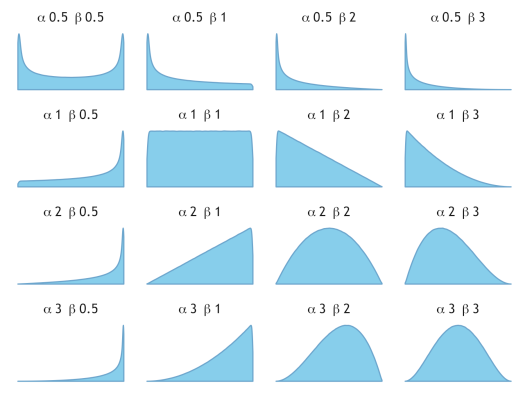
\includegraphics[scale=0.6]{beta.png}
\end{center} 
\caption{Разные формы бэта-распределения}  \label{beta_dist} 
\end{figure} 

Третий старейшина может выбрать распределение с пиком в точке $0.5$.   Например, ему подойдёт распределение с $\alpha = \beta = 2$. При разной степени уверенности, он может выбрать разную остроту пика, как следует отрегулировав параметры. Например, для $\alpha = \beta = 3$ на хвосты приходится меньше вероятностной массы. Старейшина сильнее уверен в правильности монетки. 

Мнение четвёртого старейшины можно описать с помощью $U$- образного распределения с $\alpha = \beta = 0.5$. В этом случае основная вероятностная матрица концентрируется у нуля (на монетке две решки) и у единицы (на монетке два орла). Понизив значения параметров, мы сделаем распределение ещё более резким и уберём ещё больше вероятностной массы из центра.

Мнение пятого старейшины можно выразить с помощью бимодального распределения. Например, с пиками в $0.3$ и $0.7$. $U$-образное в данном случае не подойдёт, так как оно сигнализирует именно либо о нуле, либо о единице. Для двугорбого распределения можно воспользоваться смесью двух бэта-распределений и сложить плотности, например, $\Beta(2,10)$ и $\Beta(10,2)$. Обратите внимание, сложить не случайные величины, а именно плотности. Мы хотим получить смесь из двух распределений. После складывания нужно не забыть отнормировать площадь всего этого дела к единице. 

Прогнав следующий код в R можно посмотреть как будет выглядеть сумма плотностей двух бэта-распределений. 

\begin{figure}[H]
\begin{minipage}{0.19\linewidth}
% Костыль для того, чтобы код не примыкал к правому боку
\end{minipage}
\hfill
\begin{minipage}{0.29\linewidth}
\begin{minted}{R}
library(ggplot2)
x <- seq(0,1,by = 0.001)
y1 = dbeta(x,10,2)
y2 = dbeta(x,2,10)
qplot(x,y1+y2,geom='line')
\end{minted}
\end{minipage}
\hfill
\begin{minipage}[H]{0.49\linewidth}
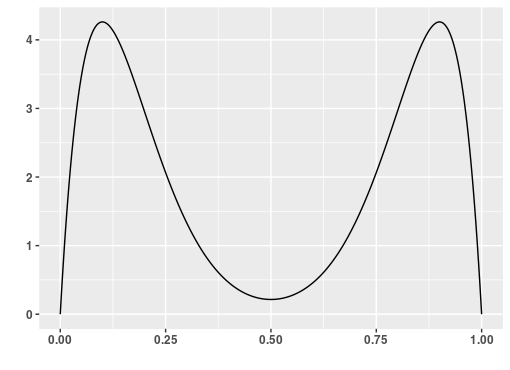
\includegraphics[scale=0.5]{beta_and_beta.png}
\end{minipage}
\end{figure}

Теперь, зная, как задаются различные априорные мнения, мы можем перейти к процедуре вероятностного вывода и посмотреть как будет выглядеть байесовская оценка для $p$ в общем случае. Пусть индейцы поиграли с испанцами в предложенную игру на что-нибудь незначительное и собрали выборку $y_1, \ldots, y_n$.  Априорно предполагается, что параметр $p$ имеет бэта-распределение, $\Beta(\alpha,\beta)$. Найдём апостериорную плотность. 

Так как  $y_1 + \ldots + y_n = n \cdot \bar{y} $, то

\begin{multline*}
f(p \mid y_1 , \ldots y_n) \propto f(y_1, \ldots, y_n \mid p) \cdot f(p) = \\ =   p^{n \bar y}(1-p)^{n-n \bar y} \cdot p^{\alpha - 1} \cdot (1-p)^{\b - 1}   = \\ =  p^{n \bar y + \alpha - 1} \cdot (1-p)^{n - n\bar y + \b - 1}. 
\end{multline*}

Уже видно, что на выходе снова получилось бэта-распределение, но с новыми параметрами. Восстановим недостающую константу

\[ const \cdot \int_0^1 p^{n \bar y + \alpha - 1} \cdot (1-p)^{n - n\bar y + \b - 1} = 1 \Rightarrow  const = \frac{1}{\Beta(n \bar y + \alpha, n-n \bar y + \beta)} \]

Параметр $p$ имеет апостериорное бэта-распределение с параметрами $n \bar y + \alpha$ и $ n - n \bar y + \beta$.  К параметру $\alpha$ прибавляется количество выпавших орлов. К параметру $\beta$ прибавляется количество выпавших решек. Априрорные значения параметров $\alpha$ и $\beta$  интерпретируются, как наша вера в правильность монеты. Чем сильнее дисбаланс между ними, тем сильнее скошена наша вера. Чем больше они, тем меньше дисперсия нашей веры. 

Попробуем использовать в качестве точечной оценки математическое ожидание апостериорного распределения. Для этого его нужно посчитать. 

	\begin{multline*}
\E(p \mid y_1, \ldots y_n)  = \\ =  \int_0^1 p \cdot \frac{1}{\Beta(n \bar y + \alpha,n-n \bar y + \b)} \cdot p^{n \bar y + \alpha - 1} (1-p)^{n - n \bar{y} + \beta - 1} dp = \\ = \int_0^1 \frac{1}{\Beta(n \bar y + \alpha ,n-n \bar y + \beta)} \cdot p^{n \bar y + \alpha + 1 - 1} (1-p)^{n - n \bar{y} + \beta - 1} dp =  \\ =   \frac{\Beta(n \bar y + \alpha + 1,n-n \bar y + \beta)}{\Beta(n \bar y + \alpha, n-n \bar y + \beta)} =  \frac{n \bar y + \alpha}{n + \alpha + \b} \cdot \frac{\Beta(n \bar y + \alpha,n-n \bar y + \beta)}{\Beta(n \bar y + \alpha, n-n \bar y + \beta)} = \\ =\frac{n \bar y + \alpha}{n + \alpha + \beta}
\end{multline*}

Выглядит внушительно. Даже пришлось немного вспомнить свойства бэта-функции.\footnote{$\Beta(q+1, p) = \frac{q}{p+q} \cdot \Beta(q,p)$}  Обратите внимание, что до этого дня никакой другой метод оценивания не давал нам такую красивую точечную оценку. Все эти вычисления с интегралами лишний раз подчёркивают, что даже в самом простом случае нам нужно обращаться к такому мощному инструменту, как бэта-функции. Очень редко попадаются случаи, когда апостериорную плотность можно найти в символьном виде. Чаще всего интегралы вообще не берутся.  

При отсутствии наблюдений получаем оценку $\frac{\alpha}{\alpha + \b}$, совпадающую с априорным математическим ожиданием. Если, наоборот, наблюдений очень много, вклад априорного мнения становится всё менее значительным и оценка приближается к среднему. 

Если при этом монетка, действительно, является односторонней, мы никогда не получим в качестве точечной оценки единицу. При каждом новом подбрасывании апостериорная оценка будет всё ближе к единице, но никогда не достигнет её.  

В каком-то смылсе байесовский способ оценивания предполагает встроенную регуляризацию\footnote{Под регуляризацией понимается накладывание дополнительных ограничение на параметры модели, которые могли бы спасти нас от переобучения, то есть от излишне сильного вылизывания обучающих данных. Об этом мы начнём по-серьёзному говорить в 5 главе и продолжим в 6.}. Если бы мы использовали на одном наблюдении метод максимального правдоподобия, мы бы получили $p=1$ и переобучились бы под выборку, сделав неправильные выводы о природе исследуемого явления. Байесовский вывод дал бы близкую к единице оценку, но не равную ей, немного застраховав нас от запоминания выборки.  Об этом мы более подробно поговорим позже.  В качестве упражнения дотошному читателю предлагается найти апостериорные оценки для каждого старейшины и сравнить их между собой.

\section{Маша, медведи и нормальное распределение}

До этого мы рассматривали ситуацию, когда наблюдения у нас дискретны, а распределение параметра непрерывно. Давайте посмотрим на ситуацию, когда непрерывны оба распределения. 

Маша прячется от Медведей в точке $m$ на числовой прямой. Есть несколько Медведей, каждый из которых обнюхивает всю числовую прямую в поисках Маши. Медведю номер $i$ кажется, что Машей сильней всего пахнет в точке $y_i$. Естественно, Медведи могут ошибаться, например, у них может быть заложен нос, поэтому $y_i \mid m \sim \mN(m, 2^2)$. При фиксированном $m$ величины $y_i$ независимы. Известно, что $y_1 = 0.5$, $y_2 = −1$.  Априорно известно, что место, где спряталась Маша имеет нормальное распределение, $m \sim \mN(1, 4^2)$. Нам нужно:

\begin{enumerate}
\item Найти апостериорную плотность распределения параметра $m$.
\item Найти апостериорные моду, медиану и математическое ожидание.
\item Найти $\PP(m > 1 \mid y_1,y_2)$.
\item Найти $f(y_3 \mid y_1,y_2)$ и $\E(y_3 \mid y_1,y_2)$.
\end{enumerate}

Целеустремлённый читатель должен сначала самостоятельно попытаться решить эту задачу, а уже после продолжить читать текст.

Посмотрим немного подробнее на наше априорное мнение о том, где сидит Маша, $m \sim \mN(1, 4^2)$. Значение $1$ в данном случае --- наше лучшее предположение о том, где она может находиться, а $2^2$, в свою очередь, это наша степень доверия к этому предположению. Чем меньшее значение дисперсии мы берём в нашем априорном мнении, тем больше наше доверие к нему.

\textbf{Делай раз! Апостериорная плотность Маши:}

\begin{multline*}
f(m \mid y_1, y_2) \propto f(y_1,y_2 \mid m) \cdot f(m) = \frac{1}{2\sqrt{2\pi}}\expp{-\frac{(0.5 - m)^2}{2 \cdot 4}} \cdot \\ \cdot \frac{1}{2\sqrt{2\pi}}\expp{-\frac{(-1 - m)^2}{2 \cdot 4}} \cdot \frac{1}{4\sqrt{2\pi}}\expp{-\frac{(m-1)^2}{2 \cdot 16}}
\end{multline*} 

Воспользуемся магической силой уже привычного нам значка $\propto$ и для простоты расчётов пренебрежём кучей констант

\[ f(m \mid y_1, y_2) \propto \expp{-\frac{(0.5 - m)^2}{2 \cdot 4}} \cdot \expp{-\frac{(-1 - m)^2}{2 \cdot 4}} \cdot \expp{-\frac{(m-1)^2}{2 \cdot 16}}\]

Сольём всё,что находится под знаком экспоненты в единое целое и попробуем упростить

\begin{multline*}
 \frac{(0.5 - m)^2}{2 \cdot 4} + \frac{(-1 - m)^2}{2 \cdot 4} + \frac{(m-1)^2}{2 \cdot 16}  = \\ = \frac{ 4(m - 0.5)^2 + 4(m+1)^2 + (m-1)^2}{32} = \frac{9m^2 + 2m + 6}{32} 
\end{multline*}

Используем двойную магию. С одной стороны пренебрегаем константой, с другой создаём новую для того, чтобы создать полный квадрат. Привыкайте пользоваться этой магией для своего удобства. Не забываем перекинуть в знаменатель лишнюю девятку

\begin{multline*}
\expp{-\frac{9m^2 + 2m + 6}{32}} \propto \expp{-\frac{9m^2 + 2m}{32}}  = \\ = \expp{-\frac{m^2+\frac{2}{9} m}{\frac{32}{9}}}  = \expp{-\frac{m^2+ 2 \cdot \frac{1}{9} m + \frac{1}{81} - \frac{1}{81}}{\frac{32}{9}}} \propto  \\ \propto  \expp{-\frac{m^2+ 2 \frac{1}{9} m + \frac{1}{81}}{\frac{32}{9}}} = \expp{-\frac{(m + \frac{1}{9})^2}{2 \cdot (\fr{4}{3})^2}}
\end{multline*}

Параметр $m$ имеет нормальное апостериорное распределение

\[m \mid y_1, y_2 \sim \mN(-\fr{1}{9},(\fr{4}{3})^2).\] 

 Обратите внимания, что после того как Медведи попытались вынюхать где находится Маша, самое вероятное её положение изменилось, а дисперсия её положения уменьшилась.

\begin{figure}[h!]
\begin{center}
\begin{tikzpicture}[scale = 1.2,
every pin edge/.style={<-},
every pin/.style={fill=yellow!50,rectangle,rounded corners=3pt,font=\small}]
\begin{axis}[every axis plot post/.append style={
  mark=none,domain=-10:10,samples=100,smooth},
clip=false,
axis y line=none,
axis x line*=bottom,
ymin=0,
xtick=\empty,
]
\addplot [blue] {\gauss{1}{2}};
\addplot [red] {\gauss{-1/9}{4/3}};

\addplot [magenta,dashed] {\gauss{0.5}{2}};
\addplot [magenta,dashed] {\gauss{-1}{2}};

\node[pin=70:{апостериорная плотность}] at (axis cs:-0.2,0.3) {};
\node[pin=70:{априорная плотность}] at (axis cs:1.5,0.19) {};
\node[pin=70:{вынюханная информация}] at (axis cs:1.9,0.1) {};
\end{axis}
\end{tikzpicture}
\end{center}
\caption{Информация  о Маше}
\end{figure}

Новая информация сместила априорную плотность влево и вытянула её вверх, в силу того, что Медведи вынюхали похожие вещи.

\textbf{Делай два!} Мода и медиана для нормального распределения совпадают с математическим ожиданием. Какую бы функцию ошибки мы не выбрали, при таком априорном мнении мы натолкнёмся на один и тот же результат.

\textbf{Делай три!} Обратите внимание, что до запуска Медведей, $\PP(m > 1) = 0.5$. После запуска, эта вероятность уменьшится,так как распределение очень сильно съедет влево.

\begin{multline*}
\PP(m > 1 \mid y_1,y_2) = 1 - \PP( m \le 1 \mid y_1,y_2) = \\ = 1 - \PP\left( \frac{m + \fr{1}{9}}{\fr{4}{3}} \le \frac{1 + \fr{1}{9}}{\fr{4}{3}} \mid  y_1, y_2 \right) = 1 - \Phi\left(\frac{10}{12}\right) \approx 0.2.
\end{multline*}


\textbf{Делай четыре!} Найдём $f(y_3 \mid y_1,y_2)$ и $\E(y_3 \mid y_1,y_2)$. Будем делать это под слоганом: <<Каждой Маше по три Медведя!>>:

\todo[inline]{Я не уверен, что то, что ниже правильно. Можно ли попроще?}

\begin{multline*}
 f(y_3 \mid y_1,y_2)  = \int_{-\infty}^{+\infty} f(y_3, m \mid y_1,y_2)\dx{m} = \\ = \int_{-\infty}^{+\infty}  f(y_3 \mid y_1,y_2,m) \cdot f(m \mid y_1,y_2) \dx{m}.
\end{multline*}

Чтобы найти плотности распределение $y_3$, мы должны провести свёртку по двум нормальным распределениям

\[ \int_{-\infty}^{+\infty} \mN(m,4)\cdot \mN \left (-\frac{1}{9},\frac{16}{9} \right)\dx{m}.\]  

Если взять этот интеграл (а мы оставляем это дотошному читателю в виде упражнения),  можно получить, что \[y_3 \mid y_1,y_2 \sim \mN \left(-\frac{1}{9},\frac{52}{9} \right).\]

Теперь, когда нюхательные способности третьего Машиного Медведя предсказаны, вы можете попробовать проделать всё то же самое самое, предположив, что вам вообще ничего неизвестно и $m \sim \mU(-\infty; +\infty)$. Именно это вам предлагается сделать в упражнении \ref{upr_norm}. Стоит отметить, что результат у вас, при этом, получится похожим на случай нормального априорного распределения с большой дисперсией. Почему это происходит именно так, мы постараемся выяснить ровно через одну главу, когда будем обсуждать энтропию.

После вы можете попытаться решить упражнение \ref{norm_upr}. Это точно такой же байесовский вывод, но для нормального распределения в общем случае. Многие формулы в этом выводе получаются довольно громоздкими. Поэтому, если вы запутатесь по ходу его самостоятельного решения, не отчаивайтесь и загляните в наше решение. В упражнении \ref{upr_predel} вас ждёт несколько прикольных асимптотических выводов, связанных с нормальными априорными распределениями. 



\section{О максимальном правдоподобии, серьёзности и бастардах}

\todo[inline]{Экспериментальный раздел, в котором я явно перегнул с аналогиями.}

Обычно, в серьёзных книгах по математике сначала формулируется теорема, а после идёт её доказательство. Если бы каждая серия Игры Престолов была бы устроена, как теорема, то в её начале томный грубый закадровый голос произносил бы длиный перечень персонажей, которые должны умереть в течение серии, а уже после показывалось бы как именно они умирают. В конце бы голос говорил: <<Все видели? А? Они умерли! Я же говорил!>>.

Почему в математике нельзя обойтись без спойлеров? Мир бы тогда был совершенно другим! В каждой книге вслед за безупречной пеленой логических рассуждений следовал бы какой-нибудь безумный факт, сносящий крышу читателя. При этом, накануне лекции недруги молодого студента, собирающегося её посетить, жадно штудировали бы книги в поисках спойлеров, а наутро, врывались бы в его комнату в общежитии и выдавали бы список из утверждений и теорем. Студент же, в свою очередь, пытался бы с зажатыми ладонями ушами добежать скорее до лекционной аудитории, чтобы увидеть оригинальные рассуждения лектора, а в конце лекции обомлеть от удивления.

В таком мире всё было бы совершенно иначе. Оценка метода максимального правдоподобия является частным случаем байесовской оценки. В качестве априорного распределения нужно взять равномерное, а в качестве точечной оценки моду апостериорного распределения. Неприятно было сейчас нарваться на такой спойлер, правда?

Чтож, теперь, зная кто умрёт в этом эпизоде, давайте заметим следущую штуку:

\[ \underbrace{f(p \mid y_1, \ldots, y_n)}_{\text{апостериорная плотность}} \propto \underbrace{f(y_1, \ldots, y_n \mid p)}_{\text{функция правдоподобия}} \cdot \underbrace{f(p)}_{\text{априорная плотность}} \]  

Если $p \sim U[0;1]$, тогда $f(p) \propto const$, значит 

\[f(p \mid y_1, \ldots y_n) \propto f(y_1 \ldots y_n \mid p).\] 

Таким образом максимум функции правдоподобия совпадает с максимумом апостериорной плотности. В свою очередь точка, где плотность достигает максимума, называется модой.
И правда, получилось,  что

\[\hat p^{ML} = \Mod(p \mid y_1, \ldots y_n). \]

Например, для случая карасей

\[ \hat p^{ML} = \bar{y} = \frac{2}{3} = \Mod f(p \mid y_1,y_2,y_3). \]

Забавно, но если мы делаем допущение, что все гипотезы априори одинаково вероятны, байесовский подход сведётся к принципу максимального правдоподобия. Результаты, полученные с помощью частотных методов являются частным случаем байесовского подхода. 

А что, если изначально гипотезы не одинаково правдоподобны априори? Получается, что в такой ситуации использование метода максимального правдоподобия приводит нас к неверным выводам? Вспомните упражнение про золотые монеты, которое вы, конечно же сделали после изучения истории про бабушку и карасей.

В этом упражнении оценка максимального правдоподобия сказала нам, что вероятность вытащить из шляпы серебряную монету равна единице. И это крайне неточно. В шляпе, из которой тянулись монетки, было несколько золотых экземпляров. Если увеличить число испытаний, то оценка станет надёжнее. Как известно, оценки максимального правдоподобия состоятельны, но, тем не менее, непонятно насколько огромным должен быть размер выборки, чтобы охватить все существующие ситуации. 

Байесовский подход позволяет в каком-то смысле избежать такой проблемы. Он говорит, что вероятность высокого значения $p$ довольно велика, но тем не менее, не отбрасывает возможность самых маленьких значений этого параметра.  Все видели? Да? А я же говорил\footnote{Авторы бы хотели отметить, что негативно относятся к спойлерам и принести свои извинения осерчавшему на них читателю. Один из авторов хотел бы передать привет одному из своих преподавателей, который в его студенчестве проспойлерил ему многие вещи из Игры Престолов. В том числе, во время зачёта по программированию, с которого автор ну никак не мог убежать с закрытыми ушами.}!

\textbf{Ещё раз, ещё раз!} Метод максимального правдоподобия --- частный случай байсовского вывода. На самом деле, довольно часто будет получаться, что какая-то вероятностная модель порождает что-то уже давно нам знакомое, настолько же знакомое, как и метод максимального правдоподобия. 

\begin{center}

\includegraphics[scale=0.6]{bayesians.jpg}
\end{center} 

Давайте для полноты картины выясним, как соотносятся между собой мода апостериорного распределения и ML-оценка при произвольном априорном распределении. Попробуйте накидать своё решение на бумажке, а после подглядите в следующую строчку со спойлерами:  

\begin{multline*}
 \Mod(\b \mid y) = \argmax_{\b} f(\b \mid y) = \\ = \argmax_{\b} f(y \mid \b) \cdot f(\b) = \argmax_{\b} (\ln f(y \mid \b) + \ln f(\b)).
 \end{multline*}

Видно, что мода апостериорного распределения, в общем случае, это коррекция $ML$ оценки. Этот факт снова наталкивает нас на мысли о регуляризации, которые будут как следует развиты в шестой главе. 


\section{Про сопряжённые распределения и сложности}

В задачах про Машу и Медведей априорное распределение было нормальным. После применения формулы Байеса мы снова получали на выходе нормальное распределение, но уже с другими параметрами. Новые параметры при этом зависели от старых параметров и собранных наблюдений.  Таким образом, чтобы получить из априорного распределения апостериорное, в данном случае не надо применять никаких сложных формул и не нужно никаких больших компьютерных мощностей. Аналогично получалось в случае бэта-распределения для монеток. Удобно.

А что если в качестве априорных распределений всегда брать такие, чтобы после домножения на правдоподобие, апостериорное распределение принадлежало тому же самому классу распределений, но с другими параметрами? Тогда бы все байесовские алгоритмы свелись бы к банальному пересчёту и всё. Конечно же мы ограничим себя в выборе априорных распределений, зато у нас не будет никаких вычислительных проблем. 

Именно так размышляли байесовцы более чем тридцать лет назад. Они решили пожертвовать своей свободой выбора в пользу простоты вычислений и нашли кучу распределений, которые ведут себя подобным образом и даже придумали для них название.

\begin{definition}
Семейство распределений $f(\beta \mid \Theta)$ называется \indef{сопряжённым по отношению к наблюдаемой выборке}, если  апостериорное распределение $f(\beta \mid y_1, \ldots, y_n)$ тоже принадлежит этому семейству. 
\end{definition}

Любопытный читатель, скорее всего, захочет узнать немножечко побольше о таких распределениях. Сделать это он может, например в статейке Айвазяна~\cite{aivaz2008}. 

Такие распределения моментально освобождали исследователя от необходимости брать сложные интегралы, решать уравнения высоких степеней, искать условные экстремумы и делать другие страшные вещи. Всё это было достаточно сделать только лишь один раз. Наши Деды позаботились о потомках, провели все эти вычисления и передали нам в наследие формулы пересчёта\footnote{На википедии можно найти целую таблицу с формулами пересчёта: \url{ https://en.wikipedia.org/wiki/Conjugate_prior}}.

Тем не менее, это обернулось для байесовского подхода лишь дополнительной критикой. В результате, в течение 20 века байесовские модели получили слабое распространение.  

В 1990-е годы произошли первые изменения. Мир вспомнил про наивный байесовский классификатор (про него мы подробно поговорим в следующей главе). Оказалось, что он иногда работает на порядок лучше, чем другие, более сложные модели. Долгое время самые простые версии таких классификаторов с очень высокой точностью защищали пользователей интернета от спама. 

Этот алгоритм называется наивным из-за того, что он допускает независимость там, где её, по гамбургскому счёту, нет. Например, в случае фильтра для спама вводится предпосылка, что вхождение слов в текст --- независимые события, что конечно же не так. Однако это работает. Видимо, для успешного выявления спама в подробности сообщения вникать не обязательно: достаточно просто уловить суть, посмотрев какие слова оно содержит. Немного позже мы обязательно обучим такой алгоритм.

В дополнение ко всему прочему, люди придумали MCMC, алгоритмы Монте-Карло по схеме Марковской цепи. Благодаря мощным компьютерам и MCMC байесовцы снова обрели свободу. Теперь, выбирая какое-то сложное априорное распределение, они не бояться случайно нарваться на убойные вычисления. Компьютер за них генерирует любые апостериорные распределения и предоставляет исследователю возможность ответить с помощью них на свои вопросы. 

Постепенно выяснилось, что байесовские методы в состоянии элегантно решать разные самые сложные задачи.  Например, совсем недавно байесовские методы скрестили с нейронными сетями. Это скрещивание открыло перед людьми колоссальные возможности. 

Одной из особенностей нейронных сетей является их самоуверенность. Если взять кучу разных картинок и случайным образом расставить на них метки, а после на этой разметке обучить свёрточную нейросеть, она запомнит какой картинке соответствует какая метка и будет на тренировочной выборке показывать превосходные результаты. При этом, на тестовой выборке, её ответы ничем не будут отличаться от случайного угадывания. Сеть никак не обучилась, не нашла никаких закономерностей и никак не сообщила об этом человеку. Она просто запомнила картинки.  \todo{Ссылка на статью}

После, для каждой новой картинки, сеть будет выдавать какой-то прогноз. Точно также она выдаст прогноз, если мы отдадим ей какую-то совершенно новую картинку, которую она никогда раньше не видела, вместо того, чтобы сказать нам, что такую картинку она видит впервые. 

Более того, сеть можно обмануть. Представим, что мы отдали ей котика а и она распознала его. В качестве ответа на нашу картинку, сеть выдала метку <<котейка>>. Возьмём ту же самую картинку с котиком, откроем её в каком-нибудь графическом редакторе и слегка подёргаем пиксели на лапке. Снова отдадим картинку нейросетке. Нейросеть спокойно может заявить нам, что это вовсе не котик, а самолёт. 

В 2015-2016 годы были предприняты первые попытки скрестить нейросети с байесовским подходом. Судя по всему, такое скрещивание позволяет решить проблему самоувернности сетей. Байесовские сети сообщают человеку насколько они уверенны в своих прогнозах. На нейросети в этой книге мы смотреть не будем. Тем не менее, кое-какие довольно новые модели постараемся пощупать.

Сейчас мы предлагаем читателю прорешать оставшиеся упражнения. Навыки байесовского вывода пригодятся нам в следующих главах.  Как говорится, Деды вычисляли! 


\section{Ещё задачи} 

\begin{problem}\label{upr1}
	
	Предположим, что вы оказались в одной из ситуаций, приведённых ниже. Как вы будете действовать?
	
	\begin{enumerate}
		
		\item Пусть мы вообще ничего не знаем о коэффициентах в модели линейной регрессии. Как мы можем замоделировать это незнание? 
		
		Другой вопрос: какое распределение можно использовать в качестве априорного, если мы знаем, что коэффициент $\beta$ принимает значение на отрезке $[\b_d; \b_u]$?
		
		\item Пусть нам необходимо оценить какой-то коэффициент в модели линейной регрессии, $\beta$. Нам точно известно, что он положительный, $\beta \in [0; +\infty)$, и, скорее всего, не принимает высокие значения. Какое распределение для параметра $\beta$ можно было бы взять в качестве априорного?
		
		\item Снова коэффициент, снова в регрессии. Теперь он точно лежит на отрезке от $0$ до $42$. Наши априорные мысли говорят, что он скорее всего ближе к $42$, чем к нулю. Как задать такое априорное распределение? 
		
		\item Джордж Мартин пишет романы из цикла <<Песнь льда и пламени>>. Пусть случайная величина $Y$ --- это число убитых в книге персонажей. Так как мы имеем дело со случайной величиной --- счётчиком, её можно было бы замоделировать с помощью распределения Пуассона с параметром $\lambda$, характеризующим частоту, с которой умирают персонажи. Какое априорное распределение можно использовать для параметра $\lambda$?
		
		\item И снова регрессия! Только теперь коэффициента два, и мы уверены, что чем больше первый, тем меньше второй. Более того, бабушка говорит, что первый должен быть в районе тройки. Про второй никто ничего не знает. Что делать? 
		
		\todo[inline]{Тут задача про смеси, которую надо переделать}
		
		%\item На числовой прямой, в некоторой точке $m$, находится месторождение нефти. Самый богатый селезень в мире хотел бы её добыть. Трое его экспертов высказывают на этот счёт свои априорные соображения. Эксперт Хьюи говорит, что $m \sim \mN(20,3)$. Эксперт Дьюи говорит, что $m \sim \mN(-20,9)$. Эксперт Луи говорит, что $m \sim \mN(0,4)$. Голова Скруджа кружится от целых трёх априорных мнений. Подскажите бедолаге, что ему делать...
	\end{enumerate}
	
\begin{sol}	
На самом деле, в описанных выше ситуациях, можно вести себя по-разному. Априорная информация сформулирована довольно размыто. Перед нами стоит задача математически точно сформулировать это размытое мнение. Можно сделать это многими разными способами. Например, авторы готовы сделать ставки на следующие распределения.

\begin{enumerate}

\item Если мы совсем ничего не знаем о параметре $\b$, то нужно брать максимально размытое распределение. Например, нормальное распределение с большой дисперсией, $\mN(0, 10^4)$. Если нам известно, что параметр $\b$ принимает значение на отрезке $[\b_d; \b_u]$, то в качестве априорного можно взять равномерное на этом отрезке распределение. Более того, в первом случае, когда $\b \in \RR$, в качестве априорного распределения можно взять $\mU(\infty; +\infty)$. Конечно, настоящего равномерного распределения на неограниченном интервале не бывает, так как 

\[ \int_{-\infty}^{+\infty} 1 \dx{x} = \infty \neq 1.\]

Такое распределение называется \indef{несобственным.} Оно говорит, что мы ничего не знаем о параметре и, что удивительно, не доставляет никаких технических неудобств. Байесовский вывод даст апостериорное распределение, пригодное для дальнейшего использования.

\item В качестве априорного распределения для коэфициента можно рассмотреть экспоненциальное, $\beta \sim Exp(-\beta)$. Область определения будет ограничена только положительными значениями. Большие значения коэффициент будет принимать с низкими вероятностями (подумайте о том может ли это побороть мультиколинеарность).

\begin{figure}[H]
\begin{minipage}[H]{0.49\linewidth}
\begin{center}
\[ f(\beta) = \begin{cases}
\exp(-\beta)&, \beta \in [0;+\infty) \\
\mbox{ } 0&, \text{иначе}\\
\end{cases} \]
\end{center}
\end{minipage}
\hfill
\begin{minipage}[H]{0.49\linewidth}
\begin{center}
\begin{tikzpicture}
% оси
\draw [->] (-1.5,0) -- (4,0);
\draw [->] (0,0) -- (0,3);
% график
\draw [blue, thick, domain=0:4] plot (\x, {1.5*exp(-1.5*\x)});
\draw [->, blue, thick] (-1.5,0)--(-0.05,0);
% точки
\draw[fill,blue] (0,1.5) circle [radius=0.03];
% подписи
\node [below] at (0,0) {0};
\node [below right] at (4,0) {$\beta$};
\node [above left] at (0,1.2) {$f(\beta)$};
\end{tikzpicture}
\end{center}
\end{minipage}
\end{figure}

Также можно выразить своё мнение с помощью любого другого стандартного распределения, обладающего необходимыми для нас свойствами. Например, подойдёт распрелеление хи-квадрат или любое другое гамма-распределение.

\item Давайте возьмём какое-нибудь известное распределение, например экспоненциальное, и перешкалируем его к отрезку $[0;42]$. Случайная величина $\b \sim Exp(\lambda)$ принимает значение на $[0;+\infty)$. Тогда Случайная величина, имеющая распределение $\frac{42}{1 + \alpha \cdot Exp(\lambda)}$ будет принимать значение как раз на требуемом отрезке! Изменяя параметр $\alpha$ можно следить за тем в какой части отрезка концентрируется подавляющая масса распределения. С помощью подобных трюков, можно модернизировать различные стандартные распределения и использовать их в качестве априорных. 

\item Параметр $\lambda$ характеризует интенсивность, с которой умирают персонажи. Мы наслышаны о том, что Джордж Мартин довольно кровожадный писатель, склонный к убийствам. Тем не менее, количество персонажей, которые погибли в течение книги не может быть слишком большим. Отсюда следует, что параметр $\lambda$ можно замоделировать распределением, сосредотачивающим основную вероятностную массу в самом начале числовой оси. Для таких целей вполне подойдёт любое гамма-распределение. Например, экспоненциальное или хи-квадрат. Параметры такого распределения, конечно же, нужно выбирать в зависимости от того насколько сильно мы верим в кровожадность Джорджа Мартина.

Кроме того, можно было предположить, что $f(\lambda) \propto \frac{1}{\lambda}$. Это распределение несобственное, но после байесовского вывода мы получим собственное апостериорное распределение.

\item Коэффициенты взаимосвязаны. Априорное распределение будет двумерным! Например, нормальным со следующими параметрами: 

\begin{equation*}
\begin{pmatrix}
\b_1 \\
\b_2
\end{pmatrix} \sim 
\begin{pmatrix}
\begin{pmatrix}
3 \\
0
\end{pmatrix} &;& \begin{pmatrix}
10^2 & & -0.2 \\
-0.2 & & 10^5 
\end{pmatrix}
\end{pmatrix}
\end{equation*}



%\item  \todo[inline]{Не уверен в корректности следующего решения}  Первое, что приходит в голову --- сформировать из трёх априорных мнений одно. Просто-напросто сложим три априорных мнения в единое и получим, что $m \sim \mN(0, 16)$. Это неправильно. При таком подходе мы потеряем абсолютно всю экспертную информацию! Мнения экспертов слишком разные. 

%Намного лучше сложить не случайные величины, а их плотности. В таком случае, мы получим трёхгорбое распределение, которое сохранит в себе особенности экспертных оценок. Прогнав следующий код в R можно посмотреть как будет выглядеть сумма экспертных плотностей. При использовании на практике, нужно будет отнормировать площадь под полученной кривой к единице.  

%\begin{figure}[H]
%\begin{minipage}[H]{0.19\linewidth}
%% Костыль для того, чтобы код не примыкал к правому боку
%\end{minipage}
%\hfill
%\begin{minipage}[H]{0.29\linewidth}
%\begin{minted}{R}
%library(ggplot2)
%x <- seq(-40,40,by=0.001)
%y1 <- dnorm(x,20,3)
%y2 <- dnorm(x,-20,9)
%y3 <- dnorm(x,0,4)
%qplot(x,y1+y2+y3,geom='l')
%\end{minted}
%\end{minipage}
%\hfill
%\begin{minipage}[H]{0.49\linewidth}
%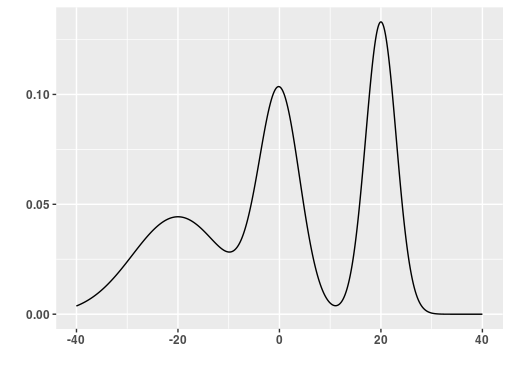
\includegraphics[scale=0.5]{makdak_norm.png}
%\end{minipage}
%\end{figure}
%
%Посудите сами, в первом случае вероятностная масса слишком сильно размазана. Нефть находится непонятно где. Во втором нефть находится в одном из горбов. В каком именно, уточнят данные. Отметим, что делая смесь из распределений, можно смешивать их с разными весами.  

%Самое байесовское решение вставшей перед Скруджем задачи состоит в последовательном пересчёте мнений. Пусть Дьюи высказал своё мнение первым. Будем считать его априорным. Мнение Хьюи рассмотрим как первое наблюдение. Воспользуемся теоремой байеса и получим апостериорное распределение. Оно впитает в себя мнение двух экспертов. Будем теперь рассматривать в качестве априорного именного его. Мнение Луи рассмотрим как новое наблюдение и снова сделаем байесовский пересчёт. Полученное после двух последовательных пересчётов апостериорное распределение впитает в себя мнения всех трёх экспертов. Именно это распределение мы будем использовать в дальнейшем как априорное. 
%
%Как это не странно, таким нехитрым образом выход одних байесовских моделей можно использовать в качестве входа к другим. Более того, вся информация о наших параметрах при таком подходе уже хранится в текущем априорном распределении. При поступлении новой информации вместо того, чтобы с нуля переоценивать все параметры модели, нам достаточно сделать простой пересчёт. Выборку, при этом, хранить в памяти необязательно. 
\end{enumerate}
\end{sol}
\end{problem}



\begin{problem}\label{upr2}
В шапке лежит куча серебрянных и золотых монет. Пусть $p$ --- доля серебряных монет. Априорно Марианне кажется, что в шляпе серебряных монет намного больше, чем золотых. Она описывает свои ожидания плотностью: 

\[ f(p) = \begin{cases}
2p&, p \in [0;1] \\
0&, \text{иначе.}\\
\end{cases} \]

Марианна тянет из шапки с возвратом монетки до тех пор, пока не вытащит серебряную. Пусть Марианна вытащила серебряную монету с первой попытки. Найдите:

\begin{enumerate}
\item Апостериорное распределение $f(p \mid~y)$;
\item $\PP(p > 0.5 \mid y)$, $\E(p \mid y)$,  $\Med(p \mid y)$,  $\Mod(p \mid y)$;
\item  $\PP(y_{new} = 1 \mid y)$;
\item Самый короткий байесовский предиктивный интервал.
\end{enumerate}
	
\begin{sol}
 Начнём с апостерионого распределения:
			
\[ f(p \mid y) =  \propto  f(y \mid p) \cdot f(p)  =   p \cdot 2 \cdot p.\]

Осталось восстановить нормировачную константу:

\[ f(p \mid y) = const \cdot p^2 \]
\[ const \cdot \int_0^1 p^2 dp = \frac{c}{3} = 1 \quad \Rightarrow \quad const = 3 \]

\begin{figure}[H]
	\begin{minipage}[H]{0.49\linewidth}
		\center Априорное распределение: \\[2.5ex]
							\begin{tikzpicture}
		% оси
		\draw [->] (-1.8,0) -- (3,0);
		\draw [->] (0,0) -- (0,3.5);
		% график
		\draw [blue, thick, domain=0:2] plot (\x, {\x});
		\draw [->, blue, thick] (-1.8,0)--(-0.05,0);
		\draw [<-, blue, thick] (2.05,0)--(3,0);
		\draw [blue, thick,dashed] (2,0)--(2,2);
		% точки
		\draw[fill,blue] (2,2) circle [radius=0.03];
		\draw[fill,blue] (0,2) circle [radius=0.03];
		% подписи
		\node [below] at (0,0) {0};
		\node [below] at (2,0) {2};
		\node [left] at (0,2) {1};
		\node [below right] at (3,0) {$p$};
		\node [left] at (0,3.3) {$f(p)$};
		\end{tikzpicture}
	\end{minipage}
	\hfill
	\begin{minipage}[H]{0.49\linewidth}
		\center Апостериорное распределение: \\[2.5ex]
		\begin{tikzpicture}
		% оси
		\draw [->] (-1.8,0) -- (3,0);
		\draw [->] (0,0) -- (0,3.5);
		% график
		\draw [blue, thick, domain=0:2] plot (\x, {1/2*\x*\x});
		\draw [->, blue, thick] (-1.8,0)--(-0.05,0);
		\draw [<-, blue, thick] (2.05,0)--(3,0);
		\draw [blue, thick,dashed] (2,0)--(2,2);
		% точки
		\draw[fill,blue] (2,2) circle [radius=0.03];
		\draw[fill,blue] (0,2) circle [radius=0.03];
		% подписи
		\node [below] at (0,0) {0};
		\node [below] at (2,0) {1};
		\node [left] at (0,2) {1};
		\node [below right] at (3,0) {$p$};
		\node [left] at (0,3.3) {$f(p)$};
		\end{tikzpicture}
	\end{minipage}
\end{figure}
		
\begin{equation*} 
\begin{aligned} 
&\PP(p > 0.5 \mid y) = \int_{0.5}^{1} 3 p^2 dp = \frac{7}{8}  \qquad \E(p \mid y) = \int_0^1 3p^3 dp = \frac{3}{4} \\ 
&\PP(p > \Med) = 0.5 \quad \Rightarrow \quad \int_0^{\Med} 3p^2 dp = 0.5 \quad \Rightarrow \quad \Med = \frac{1}{\sqrt[3]{2}} \approx 0.8 \\
&\PP(y_{new}= 1 \mid y) = \E( \PP( y_{new}= 1  \mid p,y) \mid y) = \E(p \mid y) = \frac{3}{4}.
\end{aligned}
\end{equation*}
				
Апостериорная плотность достигает своего максимума в точке $1$. $\Rightarrow \Mod(p \mid y) = 1$.
			
			
Построим самый короткий байесовский предиктивный интервал (HPD). Так как апостериорная плотность возрастает, самый короткий интервал будет примыкать к правой границе её области определения.
			
\[ \int_q^1 3p^2 dp = 0.95 \quad \Rightarrow 1 - q^3 = 0.95 \quad \Rightarrow q = \sqrt[3]{0.05} \]

Самый короткий байесовский предиктивный интервал это $[\sqrt[3]{0.05};1]$.

\end{sol}
\end{problem}


\begin{problem}\label{upr_norm}
	Та же самая задача, про ту же самую Машу, что и в главе, но у нас новое априорное распределение, $m \sim \mU(-\infty; +\infty)$. Сравните полученный результат с тем, что получалось в предыдущей задаче. А ещё найдите моду. Верно ли, что она совпадает с оценкой максимального правдоподобия? Почему? 
	\begin{sol}
		
		Получим апостериорную плотность
		
		\begin{multline*}
		 f(m \mid y_1, y_2) \propto \expp{-\frac{(0.5 - m)^2}{2 \cdot 4}} \cdot \expp{-\frac{(-1 - m)^2}{2 \cdot 4}} \propto \\ \propto \expp{-\frac{(m+0.25)^2}{2 \cdot 2}}.
		 \end{multline*}
		
		Нарисуем табличку! 
		
		\begin{table}[H]
		\begin{tabularx}{\textwidth}{XX}
			\toprule
			Априорное распределение: & Апостериорное распределение: \\
			\midrule
			$\mN(1,4^2)$             &  $\mN(-\frac{1}{9},1.77)$ \\
			$\mU(-\infty;+\infty)$   &  $\mN(-\frac{1}{4},2)$ \\
			\bottomrule
		\end{tabularx}
		\end{table}
		
		В случае, когда мы не ввели никакой априорной информации о параметре $m$, мы получили большую дисперсию, а также более сильно смещённое влево математическое ожидание. В случае, когда мы ввели априорное распределение, мы, предоставив дополнительную информацию, уменьшили дисперсию. Более того, мы не позволили вынюханным наблюдениям сдвинуть апостериорное математическое ожидание влево слишком сильно. Кстати говоря, модой будет $-0.25$.  Она действительно совпадает с  оценкой максимального правдоподобия, $\bar y$.
	\end{sol}
\end{problem}


\begin{problem}\label{norm_upr}
	
И снова Маша спряталась от Медведей в точке $m$ на числовой прямой. Есть несколько Медведей, каждый из которых пытается вынюхать где же находится Маша. Медведю номер $i$ кажется, что Машей сильнее всего пахнет в точке $y_i$. Всего у нас $n$ Медведей. Медведи могут ошибаться, например, у них может быть заложен нос, поэтому $y_i \mid m \sim \mN( m, \sigma^2)$. При фиксированном $m$ величины $y_i$ независимы. Априорно известно, что место, где спряталась Маша имеет нормальное распределение, $m \sim \mN(\mu, \tau^2)$. Найдите апостериорное распределение параметра $m$.
	
\begin{sol}

На самом деле нам нужно проделать ровно то же самое, что и для двух наблюдений. На первом шаге нужно избавиться от всех констант. На втором шаге нужно сгруппировать квадрат. Априорная плотность распределения и правдоподобие (совместная плотность распределения данных) имеют вид:

\begin{equation*}
\begin{aligned}
&f(m) = \frac{1}{\sqrt{2\pi \tau^2}} \cdot \expp{-\frac{(m - \mu)^2}{2\tau^2}} \\
&f(y \mid m, \sigma^2) = \frac{1}{(2 \pi \sigma^2)^{n/2}} \cdot \expp{-\frac{1}{2\sigma^2} \sum_{i=1}^n (y_i - m)^2}
\end{aligned}
\end{equation*}

Найдём апостериорное распределение:

\begin{multline*}
f(m \mid y, \sigma^2) \propto f(y \mid m, \sigma^2) \cdot f(m) = \\ = \frac{1}{(2\pi)^{(n+1)/2} \cdot \sigma^n \cdot \tau} \cdot \expp{-\frac{(m - \mu)^2}{2 \tau^2} - \frac{1}{2 \sigma^2} \cdot \sum_{i=1}^n (y_i - m)^2} \propto ^{*} 
\end{multline*}

Обратим внимание на то, что в нашей формуле находится куча констант, которыми можно пренебречь, а потом восстановить по аналогии с тем, как мы это делали раньше. Множитель перед экспонентой --- константа. Отбросим его. Раскроем скобки внутри экспоненты.

\begin{multline*}
^{*} \propto \expp{-\frac{m^2 - 2m \mu}{2 \tau^2} - \frac{\mu^2}{2\tau^2} - \frac{n m^2 - 2m \sum_{i=1}^n y_i}{2\sigma^2} - \frac{\sum_{i=1}^{n} y_i^2}{2\sigma^2}} \propto \\ \propto \expp{-\frac{m^2 - 2m \mu}{2 \tau^2} - \frac{n m^2 - 2m \sum_{i=1}^n y_i}{2\sigma^2} }
\end{multline*}

Обратим внимание на то, что второе и четвёртое слагаемые внутри экспоненты --- это константы, они не содержат $m$. Мы можем вытащить их в отдельный множитель и вынести за основную экспоненту. Пожертвуем ими. В оставшихся двух слагаемых везде есть случайность в виде нашего $m$. Сделаем несколько очень громоздких преобразований. Сначала приведём дроби к одному и тому же знаменателю, а затем сгруппируем скобочки.

\begin{multline*}
\frac{m^2 - 2m \mu}{2 \tau^2} + \frac{n m^2 - 2m \sum_{i=1}^n y_i}{2\sigma^2} = \\ = \frac{(\sigma^2/n) \cdot (m^2 - 2 \mu m)}{2 (\sigma^2/n) \tau^2} + \frac{\tau^2(m^2 - 2m \bar y)}{2 (\sigma^2/n) \tau^2} = \\ =  \frac{ [\sigma^2/n + \tau^2] \cdot \left[ m^2 - \frac{2\mu m(\sigma^2/n)}{\sigma^2/n+\tau^2} - \frac{2m\bar y \tau^2}{\sigma^2/n + \tau^2} \right]}{2 (\sigma^2/n) \tau^2}
\end{multline*}

Переобозначим всё, что не зависит от $m$ как константу:

\[\tilde \mu = \frac{\mu \cdot (\sigma^2/n)}{(\sigma^2/n) + \tau^2} + \frac{\bar y \cdot \tau^2}{(\sigma^2/n) + \tau^2}.\] 

Выражение выше станет более компактным:

\[ \frac{[\sigma^2/n + \tau^2] \cdot [m^2 - 2\tilde \mu \cdot m]}{2 (\sigma^2/n)\tau^2}.\]

Переобозначим ещё одну константу:


\[ \tilde \tau^2 = \frac{\tau^2 \sigma^2/n}{(\sigma^2/n) + \tau^2}.\]
 
 Всё, что находится в этой дроби снова не зависит от $m$. В итоге получаем, что

\begin{multline*} 
f(m \mid y, \sigma^2) \propto \expp{-\frac{m^2 - 2 \tilde \mu m}{2 \tilde \tau^2}} \propto  \\ \propto \expp{-\frac{m^2 - 2 \tilde \mu m + \tilde \mu^2}{2 \tilde \tau^2}} = \expp{-\frac{(m - \tilde \mu)^2}{2 \tilde \tau^2}}.
\end{multline*}

Обратите внимание, что мы дополнили числитель недостающей константой для полноты квадрата.  Мы можем себе это позволить, так как с самого начала относимся ко всем константам по-наплевательски и надеемся восстановить их в самом конце.  В итоге видим, что апостериорное распределение снова будет нормальным с параметрами $\tilde \mu$ и $\tilde \tau^2$. Решив эту задачу, мы получили две формулы для пересчёта параметров из априорного нормально распределения в апостериорное. 
\end{sol}
\end{problem}

\begin{problem}\label{upr_predel}
В предыдущей задаче\footnote{Обычно когда в книгах пишут что-то в стиле "Подставив формулу (13) в формулу (42) мы получили формулу (73). Воспользуемся ей и получим формулу (101)",  возникает нужда листать страницы до формулы (13), потом до формулы (42) и так далее, и это выбешивает. Почему нельзя напечатать эти формулы ещё раз? В этой задаче мы делаем отсылку к формулам пересчёта, полученным в предыдущей задаче. И, обратите внимание, печатаем эти формулы ещё раз, чтобы читателю было удобно и он не бросал нашу книгу. Всё для комфорта любознательного читателя!}  мы получили формулы пересчёта для параметров нормального распределения:

\[ \tilde \mu = \frac{\mu \cdot (\sigma^2/n)}{(\sigma^2/n) + \tau^2} + \frac{\bar y \cdot \tau^2}{(\sigma^2/n) + \tau^2}  \qquad \tilde \tau^2 = \frac{\tau^2 \sigma^2/n}{(\sigma^2/n) + \tau^2} \]

Получается, что апостериорное среднее это взвешенное среднее априорного распределения  и среднего по выборке, $\tilde \mu = w \cdot \mu + (1 - w) \cdot \bar{y}$. Найдите:

\begin{enumerate}
\item Предел апостериорного среднего при $\tau \to \infty$, а после при $\tau \to 0$. 
\item Предел апостериорной дисперсии при $\tau \to \infty$, а потом  при $\tau \to 0$.
\item Предел апостериорного среднего при $n \to \infty$, а также предел апостериорной дисперсии при $n \to \infty$
\item Сравните апостериорную дисперсию с априорной и с дисперсией $\bar y$.
\item Проинтерпретируйте все эти результаты. Найти-то каждый может.
\end{enumerate}

\begin{sol}
Обратите внимание, что речь в этой задаче идёт про нормальное распределение. Другие распределения ведут себя похожим образом, но не так явно. Итак, пределы $:3$

\begin{align*}
&\lim_{\tau \to \infty} \frac{\mu \cdot (\sigma^2/n)}{(\sigma^2/n) + \tau^2} + \frac{\bar y \cdot \tau^2}{(\sigma^2/n) + \tau^2} = 0 + \lim_{\tau \to \infty} \frac{\bar y}{\sigma^2/\tau^2 n + 1} = \bar y \\
&\lim_{\tau \to 0} \frac{\mu \cdot (\sigma^2/n)}{(\sigma^2/n) + \tau^2} + \frac{\bar y \cdot \tau^2}{(\sigma^2/n) + \tau^2} = \mu + \lim_{\tau \to 0} \frac{\bar y}{\sigma^2/\tau^2 n} = \mu  \\
\end{align*}

Если наша неуверенность в априорном мнении, $\tau$, очень велика, то априорная информация теряет своё значение и вес перед ней зануляется. Все выводы в таком случае мы делаем по выборке. И наоборот, если наша неуверенность в априорном мнении, $
\tau$, очень низка, то знакомство с данными никак не может изменить наши представления о значении $m$. Вес перед частью, отвечающей за выборку, зануляется.

\begin{align*}
&\lim_{\tau \to \infty} \frac{\tau^2 \sigma^2/n}{(\sigma^2/n) + \tau^2} = \lim_{\tau \to \infty} \frac{\sigma^2/n}{\sigma^2/\tau^2 n + 1} = \frac{\sigma^2}{n} \\
&\lim_{\tau \to 0} \frac{\tau^2 \sigma^2/n}{(\sigma^2/n) + \tau^2} = \lim_{\tau \to 0} \frac{\sigma^2/n}{\sigma^2/\tau^2 n + 1} = 0
\end{align*}

Если наша априорная неуверенность $\tau$ очень велика, то она теряет своё значение. Апостериорная неуверенность совпадает с дисперсией $\bar y$, а оценка с $\bar y$. И наоборот, если наша априорная неуверенность слишком мала, то наша апостериорная оценка совпадёт с $\mu$, а дисперсия окажется нулевой.

\begin{align*}
&\lim_{n \to \infty} \frac{\mu \cdot (\sigma^2/n)}{(\sigma^2/n) + \tau^2} + \frac{\bar y \cdot \tau^2}{(\sigma^2/n) + \tau^2} = \lim_{n \to \infty} \frac{\mu}{1 + \frac{\tau^2}{\sigma^2/n}} + \bar y = \bar y \\
&\lim_{n \to \infty} \frac{\tau^2 \sigma^2/n}{(\sigma^2/n) + \tau^2} = \lim_{n \to \infty} \frac{\tau^2}{1 + \dfrac{\tau^2}{\sigma^2/n}} = 0
\end{align*}

Если данных много, то они подавляют любое априорное мнение. Более того, по мере накопления данных, доверие к апостериорному распределению увеличивается и апостериорная дисперсия $\tilde \tau$  уменьшается. 

Отдельно стоит обратить внимание на то, что апостериорная дисперсия меньше как дисперсии априорного распределения, так и дисперсии $\bar y$: 

\[  \frac{\tau^2 \sigma^2/n}{(\sigma^2/n) + \tau^2} < \tau^2 \qquad \frac{\tau^2 \sigma^2/n}{(\sigma^2/n) + \tau^2} < \frac{\sigma^2}{n}. \] 

При этом 

\[ \frac{1}{\tilde{\tau}^2} = \frac{(\sigma^2/n) + \tau^2}{\tau^2 \sigma^2/n} = \frac{1}{\tau^2} + \frac{1}{\sigma^2/n}.\]

<<Точность>> апостериорного распределения равна сумме <<выборочной точности>> и <<априорной точности>>. Получается, что объединение выборочной и априорной информации приводит к увеличению <<точности>>. 
\end{sol}
\end{problem}

\begin{problem}
Вася сказал Кате, что подтягивается $7$ раз, чтобы она впечатлилась и пошла с ним на свидание, но она не поверила и послала своего младшего брата Витю проверить сколько раз подтягивается Вася. Любой парень знает, что число подтягиваний это довольно случайная штука. Васины подтягивания распределены следующим образом: 

\begin{center}
	\begin{tabular}{c|c|c|c|c|c}
		$\beta$ & 4 & 5 & 6 & 7 & 8 \\ \hline
		$\PP(\beta = k)$ & $\frac{1}{16}$ & $\frac{2}{8}$ &  $\frac{3}{4}$ &  $\frac{2}{8}$ &  $\frac{1}{16}$ \\ 
	\end{tabular}
\end{center}

Эта табличка и есть априорное мнение о том, насколько сильный из Васьки подтягун. К сожалению Витя очень невнимательный и может ошибиться в подсчётах на одно подтягивание. К счастью, он очень ответственный и знает насколько часто он ошибается: 

\begin{center}
	\begin{tabular}{c|c|c|c}
		$\varepsilon$ & -1 & 0 & 1 \\ \hline
		$\PP(\varepsilon = k)$ & $\frac{3}{8}$ & $\frac{2}{8}$ &  $\frac{3}{8}$  \\ 
	\end{tabular}
\end{center}

Итоговое число подтягиваний получается по формуле  $Y = \beta + \varepsilon$.

\begin{enumerate}
	\item Витя насчитал, что Вася подтянулся $6$ раз.  Найдите апостериорное распределение Васиных подтягиваний после подхода. 
	
	\item Из-за невнимательности Вити было решено на следующий день замерить результаты ещё раз.  Апостериорное распределение первого дня используется в качестве априорного. Витя насчитал $5$ подтягиваний. Найдите новое апостериорное распределение. 
	
	\item Предположим, что подтягуны делали подсчёты иначе. Сначала они пронаблюдали $6$ и $5$ подтягиваний, а после сделали байесовский пересчёт. Как будут отличаться результаты от случая последовательного байесовского вывода? 
	
	\item Удастся ли Ваське завоевать сердце Катьки? 
\end{enumerate} 

	\begin{sol}
\begin{enumerate}
	
	\item Параметр имеет дискретное распределение. Данные также распределены дискретно, Нам нужно получить на выходе апостериорное распределение количества подтягиваний. Подготовим почву для применения формулы Байеса и найдём нормировочную константу по формуле полной вероятности: 
	
	\[ \PP(y = 6) = \frac{3}{8} \cdot \frac{2}{8} +\frac{2}{8} \cdot \frac{3}{4} + \frac{3}{8} \cdot \frac{2}{8} = \frac{3}{8} \]
	
	Теперь нужно по формуле Байсе переоценить вероятности всех априорных гипотез. 
	
	\[ \PP(\beta = k \mid Y = 6) = \frac{\PP(y = 6 \mid \beta = k) \cdot \PP(\beta = k) }{ \PP(y=6)}\]
	
	В конечном итоге получим апостериорное распределение: 
	
	\begin{center}
		\begin{tabular}{c|c|c|c|c|c}
			$\beta$ & 4 & 5 & 6 & 7 & 8 \\ \hline
			$\PP(\beta = k)$ & $0 $ & $\frac{1}{4}$ &  $\frac{1}{2}$ &  $\frac{1}{4}$ &  $0$ \\ 
		\end{tabular}
	\end{center}
	
	Забавно, но вероятности того, что Вася подтянулся $5$ или $7$ раз не изменились, а априорная информация с хвостов перетекла в $6$ подтягиваний. 
	
	\item Посмотрим, что случится при повторном применении формулы Байеса. 
	
	\[ \PP(y = 5) = \frac{3}{8} \cdot \frac{1}{2} +\frac{2}{8} \cdot \frac{1}{4} + \frac{3}{8} \cdot  0 = \frac{1}{4} \]
	
	\begin{center}
		\begin{tabular}{c|c|c|c|c|c}
			$\beta$ & 4 & 5 & 6 & 7 & 8 \\ \hline
			$\PP(\beta = k)$ & $0 $ & $ \frac{1}{4}$ &  $ \frac{3}{4}$ &  $ 0$ &  $0$ \\ 
		\end{tabular}
	\end{center}
	
	Вероятность ещё сильнее перетекла к $6$. 
	
	\item Посмотрим, что будет, если делать пересчёт сразу же. 
	
	\[ \PP(\beta = k \mid y_1 = 6, y_2 = 5) = \frac{\PP(y = 6 \mid \beta = k) \cdot \PP(y = 5 \mid \beta = k) \cdot \PP(\beta = k) }{ \PP(y=6, y=5)}\]
	
	В этот раз не будем искать нормировочную константу влоб. Восстановим её в самом конце. 
	
	\begin{multline*}
	\PP(\beta = 6 \mid y_1 = 6, y_2 = 5) \propto \\ \propto \PP(y = 6 \mid \beta = 6) \cdot \PP(y = 5 \mid \beta = 6) \cdot \PP(\beta = 6) = \\ = \left(\frac{3}{4} \cdot \frac{2}{8} \right)\cdot \left( \frac{2}{8} \cdot \frac{3}{8} \right) \cdot \frac{2}{8} = \frac{9}{2048}
	\end{multline*}
	
	По аналогии найдём все остальные числа, пропорциональные вероятностям: 
	
	\begin{center}
		\begin{tabular}{c|c|c|c|c|c}
			$\beta$ & 4 & 5 & 6 & 7 & 8 \\ \hline
			$\PP(\beta = k)$ & $0 $ & $ \frac{9}{2048}$ &  $ \frac{12}{2048}$ &  $ 0$ &  $0$ \\ 
		\end{tabular}
	\end{center}
	
	Восстанавливаем нормировочную константу из уравнения:
	
	\[ \const \cdot ( \frac{9}{2048} + \frac{12}{2048}) = 1 \Rightarrow \const = \frac{2048}{12} \]
	
	И получаем, что итоговое распределение ничем не отличается от апостериорного распределения из предыдущего пункта.  Повторим здесь ещё раз важную мысль: выход одних байесовских моделей можно использовать в качестве входа для других. При первом выводе мы сохранили в апостериорном распределении всю информацию о наших параметрах. При втором мы её дополнили. Это эквивалентно одному большому байесовскому выводу. Это свойство оказывается полезным при масштабировании байесовских моделей на большие объемы данных. 
	
	\item Судя по всему, не получится :( 
\end{enumerate} 
	\end{sol}
\end{problem}


\begin{problem}
	
В ресторане ПушкинЪ работают два повара. Первый божественно готовит окрошку, второй ризотто.  Саша пришёл в ресторан, чтобы отобедать. Время готовки блюда $Y$ имеет экспоненциальное распределение с параметром $\alpha$.  Повара отличаются друг от друга скоростью готовки.  Для первого $\alpha = 0.1$. Для второго $\alpha = 0.2$. Работают они в ресторане день через день. Чья смена сегодня Саша не знает.  К счастью, он встретил на выходе свою подругу Наташу и успел спросить у неё как долго она ждала блюдо. Выяснилось, что $10$ минут.  Саша хочет отведать самое вкусное блюдо текущего повара. 

\begin{enumerate}
	\item  Какой из поваров готовит быстрее? 
	\item  Какое блюдо Саше нужно заказать? 
\end{enumerate}

	\begin{sol}
		Давайте вспомним природу экспоненциального распределения. Параметр $\alpha$ в нём отвечает за то, насколько тяжёлый у плотности хвост.  Более того, мы помним, что $\E(Y) = \frac{1}{\alpha}$. Для первого повара среднее значение времени готовки составит $10$ минут, для второго $20$ минут. 
		
		Повара работают день через день, значит логично было бы взять в качестве априорного распределения Саши равномерное: 
		
		\begin{center}
			\begin{tabular}{c|c|c}
				$\alpha$ & 0.1 & 0.2 \\ \hline
				$\PP(\alpha= k)$ & $0.5$ & $0.5$ \\ 
			\end{tabular}
		\end{center}
		
		Распределение дискретное. Значит апостериорное распределение также будет дискретным. Наши данные, при этом, порождаются непрерывным распределением. Наташа сказала, что ей заказ несли $10$ минут, значит функция правдоподобия будет выглядеть следующим образом: 
		
		\[ f(y \mid \alpha) = \alpha e^{-\alpha \cdot 10} \]
		
		Подготовимся к пересчёту вероятностей: 
		
		\begin{equation*}
		\begin{aligned}
		&\PP(\alpha = k \mid y) = \frac{f(y \mid \alpha = k) \cdot \PP(\alpha =k)}{f(y)} \\
		&f(y) = \PP(\alpha = 0.1) \cdot f(y \mid \alpha = 0.1) + \PP(\alpha = 0.2) \cdot f(y \mid \alpha = 0.2) \\
		&f(y) = 0.5 \cdot 0.1 e^{-0.1 y}  +  0.5 \cdot 0.2 e^{-0.2 y} \\
		\end{aligned}
		\end{equation*}
		
		
		Сделаем пересчёт вероятностей: 
		
		\begin{equation*}
		\begin{aligned}
		\PP(\alpha = 0.1 \mid y) \propto f(y \mid \alpha = 0.1) \cdot \PP(\alpha = 0.1) = 0.1 e^{-1} \cdot 0.5 \\ 
		\PP(\alpha = 0.2 \mid y) \propto  f(y \mid \alpha = 0.2) \cdot \PP(\alpha = 0.2) = 0.2 e^{-2} \cdot 0.5\\
		\end{aligned}
		\end{equation*}
		
		Последний штрих, поделим вероятности на нормировочную константу $f(y)$, которую мы восстановили выше:
		
		\begin{center}
			\begin{tabular}{c|c|c}
				$\alpha$ & 0.1 & 0.2 \\ \hline
				$\PP(\alpha= k)$ & $\frac{0.1 e^{-1}}{0.1 e^{-1} + 0.2 e^{-2}}$ & $\frac{0.2 e^{-2}}{0.1 e^{-1} + 0.2 e^{-2}}$ \\ 
			\end{tabular}
		\end{center}
		
		Или, что то же самое: 
		
		\begin{center}
			\begin{tabular}{c|c|c}
				$\alpha$ & 0.1 & 0.2 \\ \hline
				$\PP(\alpha= k)$ & $0.58$ & $0.42$ \\ 
			\end{tabular}
		\end{center}
		
		Напрашивается вывод: Саше нужно заказывать окрошку.  
		
	\end{sol}
\end{problem}


\begin{problem}
Кровожадный Джордж Мартин пишет романы из цикла <<Песнь льда и пламени>>. Кирилл совсем недавно начал знакомиться с книгами известного писателя и пока что прочитал всего-навсего $n$ книг, в каждой из которых погибло $y_1, \ldots, y_n$ персонажей. Персонажи гибнут с некоторой интенсивностью $\lambda$, то есть  $y_i \mid \lambda \sim Poiss(\lambda)$. При фиксированной интенсивности смерти персонажей в рамках одной книги не зависят от того, что написано в другой. Априорно кровожадность Джорджа Мартина описывается как $\lambda \propto \frac{1}{\lambda}$.

\begin{enumerate}
\item Найдите апостериорную условную функцию плотности $\lambda$ с учётом прочитанных книг.
\item Найдите математическое ожидание и моду для апостериорного распределения.
\item Найдите дисперсию для апостериорного распределения. Как ведёт себя дисперсия апостериорного распределения при увеличении выборки? 
\item Пусть в качестве точечной оценки Кирилл выбрал моду. Зная решение предыдущего пункта, вы бы порекомендовали ему это делать? Може быть в качестве точечной оценки лучше было бы взять математическое ожидание?
\end{enumerate}

\textbf{Hint:} для решении задачи придётся вспомнить о том, как работают гамма-функции. Не забывайте, что $ \Gamma(z) = \int_0^{+\infty} e^{-t} \cdot t^{z-1} \dx{t}$, а также, что $\Gamma(z+1) = \ z \cdot \Gamma(z)$. Также полезным может оказаться тот факт, что $\sum y_i = n \bar y$.

\begin{sol}

Продолжаем оттачивать технику байесовского вывода на новых упражнениях!

\[ f(\lambda \mid y_1, \ldots, y_n) \propto f(y_1, \dots, y_n \mid \lambda) \cdot f(\lambda) = \frac{e^{-n \cdot \lambda} \cdot \lambda^{n \cdot \bar y}}{y_1! \cdot \ldots \cdot y_n!} \cdot \frac{1}{\lambda} \propto e^{-n \cdot \lambda} \cdot \lambda^{n \bar y - 1} \]

Для того, чтобы дальше можно было бы использовать гамма-функции сделаем небольшой финт ушами:

\[ e^{-n \cdot \lambda} \cdot \lambda^{n \bar y - 1} = e^{-n \cdot \lambda} \cdot (n \cdot\lambda)^{n \bar y - 1} \cdot \frac{1}{n^{n \bar y - 1}} \propto e^{-n \cdot \lambda} \cdot (n \cdot\lambda)^{n \bar y - 1} \]

Восстанавливаем нормировочную константу.

\begin{multline*}
\const \cdot \int_0^{+\infty} e^{-n \cdot \lambda} \cdot (n \cdot\lambda)^{n \bar y - 1} \dx{\lambda} =  \\ = \frac{\const}{n}  \int_0^{+\infty} e^{-n \cdot \lambda} \cdot (n \cdot\lambda)^{n \bar y - 1} \dx{(n \lambda)} = \frac{\Gamma(n \bar y)}{n} \cdot \const = 1
\end{multline*}

Отсюда получаем апостериорное гамма-распределение:

\[ f(\lambda \mid y_1, \ldots y_n) = \frac{n}{\Gamma(n\bar y)} e^{-n \cdot \lambda} \cdot (n \cdot\lambda)^{n \bar y - 1}. \]

Найдём математическое ожидание:

\begin{multline*}
\E(\lambda \mid y_1, \ldots, y_n) = \int_0^{+\infty} \lambda \cdot \frac{n}{\Gamma(n\bar y)} e^{-n \cdot \lambda} \cdot (n \cdot\lambda)^{n \bar y - 1} \dx{\lambda} = \\ = \frac{1}{n \Gamma(n\bar y)} \int_0^{+\infty} e^{-n \cdot \lambda} \cdot (n \cdot\lambda)^{n \bar y + 1 - 1} \dx{(n \lambda)} = \frac{\Gamma(n \bar{y} + 1)}{n \Gamma(n\bar y)} = \bar y.
\end{multline*}

Найдём моду:
\begin{equation*}
e^{-n \cdot \lambda} \cdot (n \cdot\lambda)^{n \bar y - 1}  \longrightarrow \max_{\lambda} 
\end{equation*}

\begin{multline*}
-n \cdot e^{-n \cdot \lambda} \cdot (\lambda n)^{n \bar y - 1} + e^{-n \cdot \lambda} n (n \bar y - 1)(\lambda n)^{n \bar y -2} = \\ = e^{-n \cdot \lambda} (\lambda n)^{n \bar y -2} ( -n \lambda n + n (n \bar y - 1)) = 0 
\end{multline*}

\begin{equation*}
\Mod(\lambda \mid y_1, \ldots y_n) = \bar y - \frac{1}{n}.
\end{equation*}

Пришёл черёд дисперсии:

\begin{multline*}
\E(\lambda^2 \mid y_1, \ldots, y_n) = \int_0^{+\infty} \lambda^2 \cdot \frac{n}{\Gamma(n\bar y)} e^{-n \cdot \lambda} \cdot (n \cdot\lambda)^{n \bar y - 1} \dx{\lambda} = \\ = \frac{1}{n^2 \Gamma(n\bar y)} \int_0^{+\infty} e^{-n \cdot \lambda} \cdot (n \cdot\lambda)^{n \bar y + 2 - 1} \dx{(n \lambda)} = \frac{\Gamma(n \bar{y} + 2)}{n^2 \Gamma(n\bar y)}.
\end{multline*}

Раскрываем гамма-функцию:

\begin{multline*}
 \frac{\Gamma(n \bar{y} + 2)}{n^2 \Gamma(n\bar y)} = \frac{(n \bar y + 1) \cdot \Gamma(n \bar y + 1)}{n^2 \Gamma(n \bar y)} = \\ =   \frac{(n \bar y + 1) \cdot n \bar y \cdot \Gamma(n \bar y)}{n^2 \Gamma(n \bar y)} = \frac{(n \bar y + 1) \cdot n \bar y}{n^2} = \bar{y}^2 + \frac{\bar y}{n}. 
\end{multline*}

Последний штрих:

\[ \Var(\lambda \mid y_1, \ldots, y_n) = \E(\lambda^2 \mid y_1, \ldots, y_n) - (\E(\lambda \mid y_1, \ldots, y_n))^2 = \frac{\bar y}{n}.\]

Как это не странно, при увеличении выборки, дисперсия апостериорного распределения уменьшается. Наши представления о парметре $\lambda$ становятся всё более и более конкретными. При неограниченном увеличении выборки апостериорное распределение становится вырожденным. Дисперсия случайной величины сходится к нулю

\[\plim_{n \to \infty} \frac{\bar y}{n} =  \plim_{n \to \infty} \frac{\E(y_i \mid \lambda)}{n} = \plim_{n \to \infty} \frac{\lambda}{n} = 0.\]

С вероятностью единица (почти наверное) случайная величина $\lambda$ принимает своё истиное значение.

 На малых выборках мода апостериорного распределения будет давать смещённую точечную оценку.  В конечном счёте при увеличении выборки обе оценки сходятся к истиному значению параметра. Наше апостериорное распределение описывает то насколько сильно мы не знаем что происходит с параметром $\lambda$ после анализа выборки. При бесконечно большой выборке, мы знаем о параметре $\lambda$ абсолютно всё.  
\end{sol}
\end{problem}

\begin{problem}
В городе $N$ есть одна железная дорога. Эконометресса Анна Каренина каждый день в случайный момент времени приходит на вокзал города $N$ и ждёт поезд. Время, которое Аня прождала поезд, она фиксирует в своём блокноте. Известно, что поезда ходят с интервалом в $\theta$ минут, так что время ожидания поезда пассажиром можно считать случайной величиной, имеющей равномерное распределение, $y_i \sim \mU[0;\theta]$. В блокноте Ани уже есть записи $y_1,\ldots, y_n$. Аня думает, что задержка между поездами, $\theta$ не может быть очень большой. Более того, Ане кажется, что параметр $\theta$ имеет распределение Парето с плотностью: 

\begin{figure}[H]
\begin{minipage}[H]{0.39\linewidth}
\begin{center}
\[ f(\theta) = \begin{cases}
\frac{1}{\theta^2} &, \theta \ge 1 \\
0 &, \text{иначе}\\
\end{cases} \]
\end{center}
\end{minipage}
\hfill
\begin{minipage}[H]{0.59\linewidth}
\begin{center}
\begin{tikzpicture}[scale=1]
% оси
\draw [->] (-1.8,0) -- (4,0);
\draw [->] (0,0) -- (0,2);
% график
\draw [blue, thick, domain=1:4] plot (\x,{1/(\x*\x)});
\draw [->, blue, thick] (-1.8,0)--(0.95,0);
\draw [blue, thick,dashed] (1,0)--(1,1);
\draw[blue, fill=blue] (1,1) circle (0.05cm);
% подписи
\node [below] at (0,0) {0};
\node [below] at (1,0) {1};
\node [left] at (0,1) {1};
\node [below right] at (2,0) {$\theta$};
\node [above left] at (0,1.8) {$f(\theta)$};
\end{tikzpicture}
\end{center}
\end{minipage}
\end{figure}

Это означает, что Аня не верит в большие задержки. При этом, её вера убывает по степенному закону\footnote{Нассим Талеб в своей книге <<Чёрный Лебедь>> очень любит распределение Парето.}.

\begin{enumerate}
\item Существует ли в данной задаче оценка максимального правдоподобия?
\item Найдите апостериорное распределение для параметра $\theta$.
\item Найдите математическое ожидание и моду апостериорного распределения. Используйте все три точечные оценки для ответа на следующие вопросы.
\item Аня пришла на вокзал и ждала поезд $5$ минут. Как Аня оценивает время ожидания поезда? На второй  день Аня прождала поезд $2$ минуты. Как изменились Анины оценки?  На третий день Аня ждала поезд $10$ минут. Что произошло с её оценками? Какая из точечных оценок наиболее адекватно, на ваш взгляд, себя ведёт? Почему? Что при поступлении каждого нового наблюдения происходит с апостериорным распределением Ани?  
\item Нужно ли Ане срочно бросить заниматься дурью на вокзале и уйти домой, в поместье?
\end{enumerate} 
\begin{sol}
Найдём оценку максимального правдоподобия. 

\[f(y_1, \ldots, y_n \mid \theta) = \begin{cases}  \frac{1}{\theta^n}, 0 \le y_{max} \le \theta \\ 0, \text{ иначе} \end{cases}  \to \max_{\theta}.\]

Взятие производной по $\theta$ даст нам уравнение, которое нельзя решить относительно $\theta$. Мы имеем дело с нерегулярным случаем. Из-за того, что область определения случайной величины зависит от значения параметра, не выполняются условия регулярности и оценку максимального правдоподобия, в привычном для нас смысле, найти нельзя. Однако, мы можем оценить параметр на основе ограничений из выборки. Логично, что $y_1 < \theta, \ldots, y_n < \theta$. Так как функция $f(y \mid \theta)$ убывает по $\theta$, возьмём самое маленькое возможное значение этого параметра и получим, что $\theta^{ML} = y_{max}$.

Найдём для нашего параметра апостериорное распределение. Будем помнить о том, что область определения зависит от значения параметра.

\[ f(\theta \mid y) \propto f(y \mid \theta) \cdot f(\theta) = \begin{cases} \frac{1}{\theta^n} \cdot \frac{1}{\theta^2}, \theta \ge \max(y_{max},1) \\ 0, \text{ иначе} \end{cases}\]

Восстанавливаем константу: 

\[
\const \cdot \int_{\max(y_{max},1)}^{+\infty} \frac{1}{\theta^{n+2}} \dx{\theta} = 1  \Rightarrow  \const = (n+1)\cdot(\max(y_{max},1))^{n+1}
\]

На выходе получаем распределение Парето. Выглядит оно не очень удобно. Судя по форме этого распределения, его максимум достигается в самой левой точке. Значит мода будет находиться в точке $\max(y_{max},1)$. Честное взятие интеграла даст нам математическое ожидание.

\begin{tabularx}{\textwidth}{X|X|X}
Наблюдения & Математическое ожидание & Мода \\
\hline
$y_1, \ldots, y_n$ & $(1 + \frac{1}{n}) \cdot \max(y_{max},1)$ & $\max(y_{max},1)$ \\
$y_1 = 5$ & $10$ & $5$ \\
$y_1 = 5, y_2 = 2$ & $7.5$ & $5$ \\
$y_1=5, y_2=2, y_3=10$ &  $13.3$ & $10$ 
\end{tabularx}

\todo[inline]{Надо как-то переделать упражнение, чтобы появилась мораль} 

\end{sol}
\end{problem}


\begin{problem}
	Несколько упражнений на сопряжённые распределения и формулы пересчёта. 
	\begin{enumerate} 
		\item $Y \sim Bern(p)$, $p \sim \Beta(\alpha, \beta)$. Покажите, что апостериорное распределение также будет $\Beta$-распределением и выведите формулы пересчёта для параметров апостериорного распределения $\tilde{\alpha} $ и $\tilde \beta$.
		\item $Y \sim Binom(p,n)$,  $p \sim \Beta(\alpha, \beta)$. Покажите, что апостериорное распределение также будет $B$-распределением и выведите формулы пересчёта для параметров апостериорного распределения $\tilde{\alpha} $ и $\tilde \beta$.
		\item  $Y \sim Geom(p)$,  $p \sim \Beta(\alpha, \beta)$. Покажите, что апостериорное распределение также будет $B$-распределением и выведите формулы пересчёта для параметров апостериорного распределения $\tilde{\alpha} $ и $\tilde \beta$.
		\item  $Y \sim Poiss(\lambda)$, $\lambda \sim  \Gamma(s,r)$. Покажите, что апостериорное распределение также будет $\Gamma$-распределением и выведите формулы пересчёта для параметров апостериорного распределения $\tilde{s} $ и $\tilde r$.
		\item $Y \sim Exp(\alpha)$, $\alpha \sim \Gamma(s,r)$. Покажите, что апостериорное распределение также будет $\Gamma$-распределением и выведите формулы пересчёта для параметров апостериорного распределения $\tilde{s} $ и $\tilde r$.
	\end{enumerate}
	\begin{sol}
		\todo[inline]{Написать решения (или послать читателя в Айвазяна, что выгоднее)}
	\end{sol}
\end{problem}


\begin{problem}\label{upr_conf}
Пусть $f(x)$ --- плотность распределения случайной величины $X$. Исследователь Вова зафиксировал уровень значимости $\alpha$ и нашёл самый коротки доверительный интервал $[a;b]$. Известно, что у случайной величины $X$ только одна мода. Правда ли, что для этого интервала будет выполнено равенство $f(a) = f(b)$? 
\todo[inline]{Условие про одну моду лишнее или нет? Все условия учёл?} 
\begin{sol}
Разберёмся с этой задачкой двумя способами. Первый способ решения будет графическим. Пусть $f(b) > f(a)$, тогда если мы сдвинем значение $b$ вправо на $\varepsilon$, мы захватим розовый кусочек площади. 

\todo[inline]{Сделать картинку}

Для того, чтобы компенсировать вновь приобретённую площадь, значение $a$ также нужно сдвинуть вправо на значение $\delta$. Из-за того, что $f(b) > f(a)$, мы должны будем сдвинуть $a$ на большую величину, чем $\varepsilon$, чтобы компенсировать вновь появившуюся площадь. Таким образом, из-за того, что $\delta > \varepsilon$, при каждом новом сдвиге $a$ и $b$ будут сближаться друг с другом до тех пор, пока значения $f(a)$ и $f(b)$ не сравняются и мы не получим самый короткий доверительный интервал. 

\todo[inline]{Нормально описание или кривовато? Как исправить?} 

Второй способ решения будет алгебраическим. Он будет чуть более сложным. Для того, чтобы найти самый короткий доверительный интервал, мы должны решить задачку вида: 

\begin{equation*}
\left \{
\begin{aligned}
&b - a \longrightarrow \min_{a,b}  \\
&\int_a^b f(x) \dx{x} = 1 - \alpha \\
\end{aligned}
\right.
\end{equation*}

Вспомним, что $\int_a^b f(x) \dx{x} = F(b) - F(a)$ и получим, что $b = F^{-1}(\alpha + F(a))$. Подставим полученное ограничение в минимизируемую функцию

\[ F^{-1}(\alpha + F(a)) - a \to \min_a.\]

Осталась техническая часть. Берём производную обратной функции и приравниваем её к нулю. При этом, не забываем, что $y_x' = \frac{1}{x'_y}$.

За $x$ в нашей формуле обозначается $\alpha + F(a)$, за $y$ обозначается $F^{-1}(\alpha + F(a))$. Значит обратной функцией будет $F(F^{-1}(\alpha + F(a)))$. Получаем следующее уравнение

\[ \frac{1}{F'(F^{-1}(\underbrace{\alpha + F(a)}_{F(b)}))} \cdot f(a) - 1 = 0.\]

В итоге получаем, что 

\[\frac{1}{F'(b)} \cdot f(a) = 1 \quad \Rightarrow \quad f(a) = f(b).\]

Обратите внимание, что при бимодальном распределении самый короткий доверительный интервал может оказаться рваным. 

\todo[inline]{Картинка}
\end{sol}
\end{problem}


%\Closesolutionfile{solution_file}
%\input{solutions1}

\end{document}

